\documentclass{article}

\usepackage{fullpage}
\usepackage{parskip}
\usepackage{setspace}
\usepackage{mathtools}
\usepackage{tikz}
\usetikzlibrary{arrows}
\usetikzlibrary{decorations.markings}
\usetikzlibrary{calc}
\usepackage{standalone}
\usepackage{float}
\usepackage{caption}
\usepackage{subcaption}
\usepackage{amsmath}
\usepackage{amsfonts}
\usepackage{amsthm}
\usepackage[ruled]{algorithm2e}
\usepackage{adjustbox}
\usepackage{enumerate}
\usepackage{hyperref}
\usepackage[nocompress]{cite}
\usepackage{booktabs}
\usepackage{authblk}


\def\Vhrulefill{\leavevmode\leaders\hrule height 0.7ex depth \dimexpr0.4pt-0.7ex\hfill\kern0pt}

\newtheorem{definition}{Definition}
\newtheorem{theorem}{Theorem}
\newtheorem{proposition}{Proposition}
\newtheorem{lemma}{Lemma}
\newtheorem{remark}{Remark}

\title{Modelling Deadlock in Open Restricted Queueing Networks}
\author{Geraint I. Palmer}
\author{Paul R. Harper\thanks{Corresponding author Prof. Paul Harper, harper@cardiff.ac.uk}}
\author{Vincent A. Knight}
\affil{\small{\textit{School of Mathematics, Cardiff University, Senghennydd Road, Cardiff, CF24 4AG}}}
\date{\today}

\numberwithin{equation}{section}

\begin{document}

\onehalfspacing

\maketitle


\begin{abstract}
Open restricted queueing networks give rise to the phenomenon of deadlock,
whereby some customers may be unable to ever leave a server due to mutual
blocking.
This paper explores deadlock in queueing networks with limited queueing
capacity, presents a method of detecting deadlock in discrete event
simulations, and builds Markov chain models of these deadlocking networks.
The three networks for which Markov models are given include single and
multi-server networks for one and two node systems.
These models are compared to results obtained using a simulation of the
stochastic process, together with the developed deadlock detection method.
Finally, an upper bound on the expected time to deadlock of the two node
single-server network with loops is derived, by comparing its properties with
other queueing networks that are embedded within it.
This paper aims to be of value to simulation modelling of queues.

\textit{Keywords:} queues, queueing networks, deadlock, Markov models
\end{abstract}

\section{Introduction}

The study and modelling of queueing networks with blocking is an important
tool in many aspects of operational research, both analytically and through
simulation.
These models have applications in many varied settings such as healthcare,
supply chains, manufacturing and communications systems.
However, these types of models have their limitations, due to their potential
to become permanently blocked in deadlock, or a deadly embrace of resources.
These deadlocks can be real, in which case accurate modelling of deadlock is
needed, or they can occur in models where deadlock situations are easily
adjusted in reality.
In the latter case, such as by swapping two customers, a good understanding of
deadlock is needed in order to model the adjusted reality.

Queueing networks are described as open if customers can enter and leave the
system from the exterior.
Restricted networks are those where at least one service centre has limited
queueing space or capacity before it.
Deadlock is caused by blocking.
This paper considers Type I blocking: after service a customer will be blocked
from joining a queue at another node if that node's queueing capacity is full.
While blocked, that customer remains with its server until space becomes
available at its destination.
During this time that server is unavailable to begin another customer's
service.

For the purposes of this paper, deadlock is defined as follows.\\

\begin{definition}
    A queueing network is in deadlock when at least one service station
    permanently ceases to begin of finish any more services, due to circular
    blocking.
    That is, when there is a subset of blocked customers $B$ who are blocked,
    directly or indirectly, by other customers in $B$ only.
\end{definition}


Figure~\ref{fig:1st_example} shows an open two node restricted queueing
network in deadlock.
The customer at the top server is blocked from entering the bottom node as
there is a full queue, and similarly the customer at the bottom server is
blocked from entering the top node as there is a full queue.
It is clear that by following the rules of a blocking defined above, no more
natural movement can happen.

\begin{figure}[!htbp]
  \begin{center}
  \includestandalone[width=0.4\textwidth]{images/2nodesindeadlock}
  \end{center}
  \caption{Example of an open two node restricted queueing network in deadlock.}
  \label{fig:1st_example}
\end{figure}

This paper is concerned with open restricted queueing networks that experience
Type I blocking.
Throughout the paper service centres will be referred to as nodes, and for the
$i$th node of an open restricted queueing network the following notation is
used:

\begin{itemize}
  \item $\Lambda_i$ denotes the external arrival rate.
  \item $\mu_i$ denotes the service rate.
  \item $c_i$ denotes the number of parallel servers.
  \item $n_i$ denotes the queueing capacity.
  \item $r_{ij}$ denotes the routing probability from node $i$ to node $j$
  upon completion of service at node $i$.
\end{itemize}

Exponential service times and Poisson arrivals are assumed.

In particular this paper looks at detecting when deadlock occurs, and the time
until a deadlock occurs from an empty system.
First, a method for detecting deadlock in simulations of queueing networks is
presented.
Then, Markov models of simple deadlocking queueing networks are built.

The remainder of this paper is structured as follows:
Section~\ref{sec:motivatingexample} gives a motivating example to put the work
in context.
Section~\ref{sec:litreview} gives an overview of existing literature on the
subject.
Section~\ref{sec:detectingdeadlock} presents a method of detecting deadlock in
simulations of queueing networks.
Section~\ref{sec:markovmodels} presents Markov models of three deadlocking
queueing networks, derives their expected time to deadlock, and compares these
with results obtained through the simulation model.
Finally Section~\ref{sec:bound} derives a bound for the expected time to
deadlock for one of the queueing networks discussed.




\section{A Motivating Example}\label{sec:motivatingexample}

Here we present a motivating example of a healthcare system.
In this example, deadlock would not be reached in reality, however using
stochastic modelling and simulation the model would exhibit deadlock.
Therefore and understanding of this phenomenon, and an ability to overcome
this effect is discrete event simulations, is essential for modelling this
system.

Consider the interface between secondary care services at a hospital and
community care services.
Patients can be admitted to hospital via a variety of routes (through
emergency services, outpatients), and via referral from community care
services.
Patients can begin receiving community care packages due to referral from GP,
or via referral from the hospital.
Considering only the hospital and community care services as nodes, this
system is shown in Figure~\ref{fig:motivatingexample}.

\begin{figure}
\begin{center}
\includestandalone[width=0.6\textwidth]{images/motivatingexample}
\end{center}
\caption{Diagram of patient flows at an interface between secondary care
services at a hospital and community care services.}
\label{fig:motivatingexample}
\end{figure}

If there are no free hospital beds, then patients being referred from
community care services will be sustained by community care workers until beds
become available.
If there are no community care packages available, then patients requiring
packages but unfit to return home after a hospital stay will remain in
hospital, blocking beds until a community care package becomes available.
Type I blocking occurs here, as patients and staff do not know the future
capacity of their next destination prior to service.

In this model there is a non-zero probability of everyone at the hospital
blocking beds waiting for community care packages, and everyone at community
care being sustained waiting for beds at the hospital.
Thus the model will exhibit deadlock.
In reality, there is communication between there services and patients can
swap places.
This ensures no deadlock.
An understanding of how deadlock behaves in the model, and a deadlock
detection method in the simulation model will ensure correct models can be
built of systems like this with circular blocking.

Restricted feedback loops that exhibit mutual blocking such as this one have
been observed in real healthcare systems, as described in a case study in
\cite{osoriobierlaire09}.
However, just as in this motivating example, the authors here state that this
type of blocking ``may be irrelevant in practice given that the swapping of
patients can be identified and carried out easily''.
This emphasises the discrepancies that occur between common modelling
techniques and reality in systems that may reach deadlock.


\section{Literature Review}\label{sec:litreview}

Restricted queueing networks that exhibit blocking are well discussed in the
literature, both exact \cite{hunt56, baber08, aviitzhakyadin65, koizumietal05,
latoucheneuts80, perrosetal88, gordonnewell67} and approximate methods
\cite{takahashi80, korporaaletal00, onvural90, perrosetal88, dalleryfrein93,
allonetal13, osoriobierlaire09}.
Discussions on restricted queueing networks with feedback loops, that may
exhibit deadlock, are sparse however.
In fact the problem of deadlock in queueing networks has either been ignored,
not studied, or assumed resolved in much of the literature \cite{onvural90,
perrosetal88, osoriobierlaire09}.

Central to the study of deadlock in queueing networks is the concept of
blocking.
In \cite{onvuralperros86} three types of blocking are described.
Type I blocking (blocked at service, BAS, transfer blocking) occurs when a
customer is blocked after completing service, and remains with the server
until capacity at their destination node becomes available.
Type II blocking (blocked before service, BBS, service blocking) occurs when a
customer declares their destination before beginning service, and is only
granted service if there is available capacity at their destination node.
In Type III blocking (repetitive services, RS-FD and RS-RD, rejection
blocking) instead of getting blocked a customer is required to repeat their
service if there is no capacity at their destination.
This type of blocking comes in two forms, fixed destination where the
customer's destination does not change at each repetition of service, and
random destination, where the customer's destination is re-sampled from a
probability distribution after each repetition.

There has been a body of research into detection and prevention of deadlock
which doesn't consider the underlying stochastic structure of the system
\cite{coffmanelphick71, reveliotis15a, reveliotis15b}.
These general deadlocks occur in flexible manufacturing systems and
distributed communication systems.
This type of deadlock, also referred to as deadly embraces
\cite{coffmanelphick71}, can potentially occur under the following conditions:
\begin{itemize}
  \item Mutual exclusion: Tasks have exclusive control over resources.
  \item Wait for: Tasks do not release resources while waiting for other
  resources.
  \item No pre-emption: Resources cannot be removed until they have been used
  to completion.
  \item Circular wait: A circular chain of tasks exists, where each task
  requests a resource from another task in the chain.
\end{itemize}

In open restricted queueing networks the mutual exclusion condition is
satisfied as customers cannot share servers; the wait for condition is
satisfied due to the blocking rules defined previously; the no pre-emption
condition is satisfied in networks that have no or non-pre-emptive priority
(this paper only considers networks with no priority); and the circular wait
condition is satisfied if the queueing network contains a cycle where all
nodes have limited queueing capacity, that is, a feedback loop.

Allowing a system to reach deadlock can be problematic in cases where
automated systems cannot continue operations, or where simulations cannot
accurately model reality.
In general there are three strategies for dealing with the problem of deadlock
\cite{kawadkaretal14, elmagarmid86, venkateshsmith05, vis06}:

\begin{itemize}
  \item Avoidance, in which decisions are made as time unfolds to avoid
  reaching deadlock.
  \item Prevention, in which the system is designed such that in cannot
  possibly deadlock in the first place.
  \item Detection and recovery.
\end{itemize}

Note that \cite{holt72} lists the three strategies as prevention, detection
and crashing, which is equivalent to having no deadlock strategy.
Allowing the system to crash now and again may be more economical in some
systems where deadlocks do not occur often enough to justify the investment
and effort of implementing an avoidance/resolution strategy.

The first two of these strategies, prevention and avoidance, have been used
extensively in an area known as Discrete Event Systems (DES)
\cite{reveliotis15a, reveliotis15b}.
A distinction between \textit{online} and \textit{offline} resource allocation
strategies is made \cite{venkateshsmith05}.
Deadlock avoidance techniques are online strategies, decisions are made as the
system runs, whereas deadlock prevention techniques are offline strategies as
decisions are made in the planning and designing of the system.

Various techniques and methods have been used to implement deadlock avoidance
such as the Banker's algorithm \cite{dijkstra82, kawadkaretal14}, petri net
models \cite{viswanadhametal90, ezpeletaetal02, marchettimunierkordon09}, and
resource allocation graphs \cite{belik90}.
A survey of avoidance techniques for automated guided vehicle systems is given
in \cite{vis06}.
These techniques generally determine when resources cannot be allocated as
that allocation would lead to deadlock.
In \cite{florianetal08} a priority based deadlock avoidance algorithm is
implemented in a traffic simulation model.
The purpose of the avoidance scheme here is not to reflect deadlock avoidance
in reality, but to avoid deadlocks that will occur in the simulation due to
missing information or incomplete models.

The literature has discussed deadlock prevention in closed queueing networks
when blocking of Type I occurs.
For closed networks of $K$ customers with only one class of customer,
\cite{kunduakyildiz89} proves the following condition to ensures no deadlock:
given that each node $j$ has total capacity $B_j$, for each minimum cycle $C$,
$K < \sum_{j\in C} B_j$, the total number of customers cannot exceed the total
queueing capacity of each minimum sub-cycle of the network.
The paper also presents algorithms for finding the minimum queueing space
required to ensure deadlock never occurs for closed cactus networks, where no
two cycles have more than one node in common.
This result is extended to multiple classes of customer in
\cite{liebeherrakyildiz95}, with more restrictions such as single servers, and
each class having the same service time distribution.
Here a integer linear program is formulated to find the minimum queueing space
assignment that prevents deadlock.

Further conditions on deadlock prevention in closed queueing networks are
reviewed in \cite{onvural90}, including closed networks under different
blocking mechanisms such Type II and Type III blocking.
For simulation modelling however, prevention and avoidance techniques may not
be appropriate as they can potentially inhibit realism in the simulation by
taking actions that do not occur in the system being modelled
\cite{venkateshetal98}.

In \cite{schmidtjackman00} a deadlock prevention/avoidance mechanism for open
restricted queueing networks is given.
Here, arrivals from outside the system are turned away if certain nodes are
full.
This ensures that the whole system cannot become saturated, and reach deadlock.

A popular method of detecting general deadlock is the use of wait-for graphs,
state-graphs and other variants \cite{cheng90, elmagarmid86, coffmanelphick71,
choetal95, deuermeyeretal97, venkateshetal98, venkateshsmith03,
venkateshsmith05, holt72}.
These wait-for graphs, keep track of all circular wait relations between tasks.
In \cite{coffmanelphick71} dynamic state-graphs are defined with resources as
vertices and requests as edges.
For scenarios where there is only one type of each resource, deadlock arises
if and only if the state-graph contains a cycle.
In \cite{choetal95} `simple bounded circuits' are defined by giving the
vertices and edges of the state graph labels in relation to a reference node.
The existence of these circuits within the state graph indicates if the system
is in deadlock.
A strategy of this type is developed in this paper to detect deadlock in
queueing systems.

Bipartite graphs are used in \cite{holt72} to detect deadlock in systems with
both consumable and reusable resources, where the concept of reducibility and
knots are used to detect deadlock in certain situations.
These graphs are developed and used in \cite{deuermeyeretal97} and
\cite{venkateshsmith03} where these dynamic bipartite entity-resource graphs
(E/R graphs) are used to detect two different types of deadlock, transient
deadlock and permanent deadlock. A deadlock resolution procedure is proposed
that attempts to break cycles in the E/R graph
These E/R graphs contain resources and entities as vertices, and request or
holding relationships as edges; strongly connected components and closed
strongly connected components indicate a deadlock situation.
This work is furthered in \cite{venkateshetal98} where deadlock is detected
and resolved for situations where entities may request more than one resource.

A number of deadlock types are defined in \cite{venkateshetal98}, and their
relationships to one another.
This is shown in Figure~\ref{fig:deadlocktypes}.
`Transient deadlock' defined there corresponds to the blocking considered in
this manuscript, and isn't considered a deadlock situation here; whereas
`permanent deadlock' and `absolute deadlock' defined there is equivalent to
the type of deadlock that is discussed in this paper.
The authors of \cite{venkateshetal98} state that in overlapping deadlock
situations (the kind that arise in the queueing networks discussed in this
paper) there is no conceptual difference between transient and permanent
deadlocks, however using the definitions given in this paper transient
deadlock is not considered a deadlock at all, and thus we consider these two
deadlock situations as fundamentally different.

\begin{figure}[!htbp]
  \begin{center}
  \includestandalone[width=0.9\textwidth]{images/deadlockdiffliterature}
  \end{center}
  \caption{Illustrating the types of deadlock, and the differences between the
  meaning of deadlock in this paper (top writing) and in some of the
  literature (bottom writing). Adapted from \cite{venkateshetal98}.
  States considered as deadlock are italicised.}
  \label{fig:deadlocktypes}
\end{figure}

Deadlock detection and recovery in closed queueing networks through swapping
customers is assumed in \cite{perrosetal88}, with zero transition time assumed
between deadlocked states and the corresponding resolved state.
Time to resolve deadlock may not be negligible in reality.
Deadlock detection and recovery is listed as one of the two possible solutions
for handling deadlock in queueing networks in \cite{akyildiz89}, although
there is no further discussion.





\section{Deadlock Detection}\label{sec:detectingdeadlock}

In order to detect when deadlock has occurred in a queueing network
simulation, a state digraph is used, a form of wait-for graph.
In previous literature on wait-for graphs these are bespoke graphs that
represent system states, where edges denote some form of waiting or blockage
relationships.
Here we present a generic state digraph that is defined for all FIFO
queueing networks that exhibit Type I blocking:


\begin{definition}
The state digraph $D(t)$ of a queueing network is defined by that network's
state at any time $t$.
Vertices of the state digraph correspond to servers of the network.
A directed edge denotes a blockage relationship in the following manner: if a
customer at the $k$th server of node $i$ is blocked from entering node $j$,
then there are directed edges from the vertex corresponding to node $i$'s
$k$th server to every vertex corresponding to the servers of node $j$.
\end{definition}

To illustrate this concept Figure~\ref{fig:exampledigraphs} shows examples of
queueing networks in and out of deadlock, and the corresponding state digraph
in each case.

\begin{figure}[!htbp]
\begin{center}
  \begin{subfigure}{0.45\textwidth}
    \begin{center}
      \includestandalone[width=0.8\textwidth]{images/exampledigraph_1}
    \end{center}
    \caption{A three node queueing network in deadlock, with state digraph.}
    \label{fig:exampledigraph_deadlock}
  \end{subfigure}
  \hspace{6 mm}
  \begin{subfigure}{0.45\textwidth}
    \begin{center}
      \includestandalone[width=0.8\textwidth]{images/exampledigraph_2}
    \end{center}
    \caption{A three node queueing network not in deadlock, with state
    digraph.}
    \label{fig:exampledigraph_nodeadlock}
    \vspace{6 mm}
  \end{subfigure}
  \begin{subfigure}{0.45\textwidth}
    \begin{center}
      \includestandalone[width=0.8\textwidth]{images/exampledigraph_3}
    \end{center}
    \caption{A two node queueing network in deadlock, with state digraph.}
    \label{fig:exampledigraph2_nodeadlock}
  \end{subfigure}
  \hspace{6 mm}
  \begin{subfigure}{0.45\textwidth}
    \begin{center}
      \includestandalone[width=0.8\textwidth]{images/exampledigraph_4}
    \end{center}
    \caption{A two node queueing network not in deadlock, with state digraph.}
    \label{fig:exampledigraph2_nodeadlock}
    \vspace{6 mm}
  \end{subfigure}
  \end{center}
  \caption{Examples of state digraphs with their corresponding queueing
  networks.}
  \label{fig:exampledigraphs}
\end{figure}

These graph theoretic terms will be used throughout this paper
\cite{gibbons85, wilson70}:

\begin{itemize}
  \item Two vertices $v_1$ and $v_2$ are said to be \textit{strongly
  connected} if there is a directed path from $v_1$ to $v_2$ and a directed
  path from $v_2$ to $v_1$.
  \item Two vertices $v_1$ and $v_2$ are said to be \textit{weakly connected}
  if there is either a directed path from $v_1$ to $v_2$ or a directed path
  from $v_2$ to $v_1$.
  \item A \textit{strongly connected component} of a digraph is a subgraph
  induced by a maximal subset of strongly connected nodes.
  \item A \textit{weakly connected component} of a digraph is a subgraph
  induced by a maximal subset of weakly connected nodes.
  \item $v_1$ is an \textit{ancestor} of $v_2$ if there is a path from $v_1$
  to $v_2$.
  \item $v_2$ is a \textit{descendant} of $v_1$ if $v_1$ is an ancestor of
  $v_2$.
  \item The \textit{in-degree} of $v_1$, denoted $\text{deg}^{\text{in}}(v_1)$
  is the number of in-edges incident to $v_1$.
  Similarly the \textit{out-degree} of $v_1$, denoted
  $\text{deg}^{\text{out}}(v_1)$ is the number of out-edges incident to $v_1$.
  \item A \textit{source} is a vertex whose in-degree is zero.
  A \textit{sink} is a vertex whose out-degree is zero.
\end{itemize}

Consider one weakly connected component $G(t)$ of $D(t)$ and a node
$X \in G(t)$. Some observations:

\begin{itemize}

  \item If the server corresponding to $X$ is unoccupied, then $X$ has no
  incident edges.
  \item Consider the case when the server corresponding to $X$ is occupied by
  individual $a$, whose next destination is node $j$.
  Then $X$'s direct successors correspond to servers occupied by individuals
  who are blocked or in service at node $j$.
  \item It can interpreted that all $X$'s descendants correspond to servers
  whose occupants are directly or indirectly blocking $a$, and interpret all
  $X$'s ancestors as those servers whose individuals are being blocked
  directly or indirectly by $a$.
  \item All vertices of $G(t)$ are either descendants of another vertex, and
  so correspond to servers occupied by an individual who is blocking someone;
  or are ancestors of another vertex, and so are occupied by someone who is
  blocked.
  \item Note that the only possibilities for $\text{deg}^{\text{out}}(X)$ are
  0 or $c_j$. If $\text{deg}^{\text{out}}(X) = c_j$ then $a$ is blocked by all
  its direct successors. The only other situation is that $a$ is not blocked,
  and $X \in G(t)$ because $a$ is in service at $X$ and blocking other
  individuals, in which case $\text{deg}^{\text{out}}(X) = 0$.
  \item It is clear that if all of $X$'s descendants correspond to servers
  occupied by blocked individuals, then the system is deadlocked at time $t$.
  \item By definition all of $X$'s ancestors correspond to servers occupied by
  blocked individuals.

\end{itemize}

Recall that a knot is defined as a strongly connected component where no
vertex has a path to any vertices not in that strongly connected component.
Therefore there can be no path from a vertex in the knot to a vertex without
any out-edges.
The following results detect deadlock for open restricted queueing networks.


\begin{theorem}\label{thrm:knot}
A deadlocked state arises at time $t$ if and only if $D(t)$ contains a knot.
\end{theorem}

\begin{proof}{Proof}
Consider one weakly connected component $G(t)$ of $D(t)$ at time $t$.

Assume that $G(t)$ contains a vertex $X$ such that
$\text{deg}^{\text{out}}(X) = 0$, and there is a path from every other
non-sink vertex to $X$.
This implies that $X$'s occupant is not blocked and is a descendant of another
vertex.
Therefore the queueing network is not deadlocked as there does not exist a
vertex whose descendants are all blocked.

Now assume that we have deadlock.
For a vertex $X$ which corresponds to a server involved in the deadlock, all
descendants of $X$ are are occupied by individuals who are blocked, and so
must have out-degrees greater than 0.
And so there is no path from $X$ to a vertex with out-degree of 0.

\end{proof}

The knot condition can be simplified for specific cases.

\begin{proposition}
For queueing networks:
\begin{enumerate}
  \item with one node
  \item with two nodes, each with two or fewer parallel servers
  \item with a finite amount of nodes, each with a single-server
\end{enumerate}
a deadlocked state arises if and only if there exists a weakly connected
component without a sink node.
\end{proposition}

\begin{proof}{Proof}
  There are three parts to this proof:

  \begin{enumerate}

  \item
  Consider a one node queueing network.

  If there is deadlock, then all servers are occupied by blocked individuals,
  and so all servers have an out-edge.

  \item
  Consider a two node queueing network, each node with 2 or fewer parallel
  servers.

  If both nodes are involved in the deadlock, so there is at least one
  customer in node 1 blocked from entering node 2, and at least one customer
  from node 2 blocked from entering node 1, then all servers in node 1 and
  node 2 in $D(t)$ will have out edges as they are occupied by a blocked
  individual.
  The servers of node 1 and 2 consist of the entirety of $D(t)$, and so there
  is no sink nodes.

  Now consider the case when only one node is involved in the deadlock.
  Without loss of generality, consider that node 1 is in deadlock with itself,
  then the servers of node 1 have out-edges.
  For the servers of node 2 to be part of that weakly connected component,
  there either needs to be an edge from a server in node 1 to a server in node
  2, or an edge from a server in node 2 to a server in node 1.
  An edge from a server in node 1 to a server in node 2 implies that a
  customer from node 1 is blocked from entering node 2, and so node 1 is not
  in deadlock with itself.
  An edge from a server in node 2 to a server in node 1 implies that a
  customer in node 2 is blocked from entering node 1.
  In this case one server in node 2 has an out-edge.
  Now either the other server of node two is empty or still in service, and so
  isn't part of that weakly connected component, or the other server's
  customer is blocked and so has an out edge.

  For the case of a two node queueing network with at least one node with more
  than 2 servers, consider the following counter-example:

  Node $A$ has two parallel servers, node $B$ has three parallel servers.
  Begin with all servers occupied by customers in service and full queues.
  The customer at server $A_1$ is blocked to node $A$.
  The customer at server $B_1$ is blocked to node $A$.
  The customer at server $B_2$ is blocked to node $B$.
  The customer at server $A_2$ is blocked to node $A$.
  Node $A$ is a deadlocked.
  The resulting state digraph in Figure~\ref{fig:counter_example_1} has a
  weakly connected component with a sink.

  \item
  Consider a queueing network with $N$ nodes, each with a single-server.

  If $1 \leq n \leq N$ nodes are involved in the deadlock, then each server in
  those $n$ nodes has a blocked customer, and so has an out-edge.
  Of the other nodes, they can only be in the same weakly connected component
  if either they contain a blocked individual, in which case they will have an
  out edge; or they are blocking someone who is blocked directly or indirectly
  by those in deadlock.
  However this last case cannot happen, as every node is single-server each
  person can only be blocked by one other individual at a time.

  For the case of a queueing network with more than two nodes with multiple
  servers, the following counter-example proves the claim:

  Node $A$ has one parallel server, node $B$ has two parallel servers, and
  node $C$ has two parallel servers.
  Begin with all servers occupied by customers in service and full queues.
  The customer at server $B_1$ is blocked from entering node $A$.
  Then the customer at server $C_1$ is blocked from entering node $B$.
  Then the customer at server $A_1$ is blocked from entering node $A$.
  Node $A$ is deadlocked.
  The resulting state digraph in Figure~\ref{fig:counter_example_2} has a
  weakly connected component with a sink.
  \end{enumerate}
\end{proof}

\begin{figure}
\begin{subfigure}{0.5\textwidth}
\begin{center}
\includestandalone[width=0.8\textwidth]{images/counter_example_digraph_1}
\end{center}
\caption{State Digraph of Counter-Example 1.}
\label{fig:counter_example_1}
\end{subfigure}
\begin{subfigure}{0.5\textwidth}
\begin{center}
\includestandalone[width=0.65\textwidth]{images/counter_example_digraph_2}
\end{center}
\caption{State Digraph of Counter-Example 2.}
\label{fig:counter_example_2}
\end{subfigure}
\caption{Counter examples.}
\label{fig:counter_examples}
\end{figure}


For the purposes of this paper, a simulation model is used to verify that the
results of this section and the analytical model in
Section~\ref{sec:markovmodels} are in agreement.
Specifically the time taken to reach deadlock from an empty system is
investigated, and the simulation model gives information on the distribution
of times to deadlock.
The model is built using Ciw \cite{ciwpython}.
This is an object oriented framework in Python \cite{python15}, with care
taken to ensure reproducibility of the results \cite{hongetal15}.

The digraph \(D(t)\) is implemented as an attribute of the queueing network
and is updated at the appropriate events.
Note that a brute force algorithm is used to check whether each strongly
connected component of $D(t)$ is a knot in order to implement
Theorem~\ref{thrm:knot}.
More efficient algorithms could be used for other specific use cases.

The next section builds Markov models of five queueing networks, and discusses
their deadlocking properties.


\section{Markovian Models of Deadlocking Queueing Networks}\label{sec:markovmodels}

The following three networks describe all possible configurations of 
deadlocking queueing networks with two or fewer nodes:

\begin{enumerate}
  \item Open one node, multi-server restricted queueing network with feedback
  loop. (Section~\ref{sec:1nodeMS}) \label{itm:1Nms}
  \item Open two node, multi-server restricted queueing network with routes
  between nodes. (Section~\ref{sec:2nodeMS}) \label{itm:2Nmss}
  \item Open two node, multi-server restricted queueing network with routes
  between nodes and self-loops. \label{itm:2Nmsf}
\end{enumerate}

In this section Markov models are built for networks~\ref{itm:1Nms} and
\ref{itm:2Nmss}, and expressions for their expected time to deadlock found.
The state space for network~\ref{itm:2Nmsf} is too large to model in a similar
way to the others, and so isn't considered in this paper.
A single server version is modelled however, and the multi-server system will
be discussed in Section~\ref{sec:conclusions}.
In Section~\ref{sec:bound} a relationship (a bound) is given between single
server versions of network~\ref{itm:2Nmsf} and networks~\ref{itm:1Nms}
and~\ref{itm:2Nmss}.

In general a continuous Markov chain model of a deadlocking queueing network
is defined by a set of states $s \in S$ and the transition rates between these
states $q_{s_1,s_2}$.
Each state $s$ uniquely defines a configuration of customers around the
queueing network.
Deadlocked states are also present, either denoted by that specific
configuration of customers, or by negative numbers, for example (-1).
Deadlocked states cannot transition to any other state, and so are absorbing
states of the Markov chain.
Therefore any queueing network that can experience deadlock is guaranteed to
experience deadlock, as absorbing Markov chains are guaranteed to enter one of
its absorbing states.

The expected time until deadlock is reached is equivalent to the expected time
to absorption of the Markov chain, which can easily be found \cite{stewart09}.
The canonical form of an absorbing Markov chain is

\begin{equation*}
P = \left(\begin{array}{cc} T & U\\ 0 & I \end{array} \right)
\end{equation*}

where $I$ is the identity matrix.

Now the expected number of time steps until absorption starting from state $i$
is the $i\text{th}$ element of the vector

\begin{equation} \label{eq:abs_probs}
  (I - T)^{-1}e
\end{equation}

where $e$ is a vector of 1s.

Therefore by discretising the continuous Markov chain and ensuring the correct
order of states, the expected number of time steps to absorption, which
corresponds to deadlock, can be found.

When there is more than one deadlocked state, there is more than one absorbing
state in the Markov chain.
Here the expected time to absorption is the expected time to a deadlocked
state, whichever one that may be.
The probabilities of which absorbing state a Markov chain will reach are given
by the $(i, j)^{\text{th}}$ element of the following matrix:

\begin{equation}
  (I - T)^{-1}U
\end{equation}

which corresponds to the probability of reaching absorbing state $j$ from
transient state $i$.


\subsection{One Node Multi-Server}\label{sec:1nodeMS}


Consider the open one node multi-server restricted queueing network shown in
Figure~\ref{fig:queueingnetwork_1nodemulti}.
This shows an \(M/M/c/n\) queue where customers arrive at a rate of $\Lambda$
and served at a rate $\mu$.
Once a customer has finished service they rejoin the queue with probability
$r_{11}$, and so exit the system with probability $1 - r_{11}$.
Let this system be denoted by $\Omega_1$ with parameter set $(\Lambda$, $\mu$,
$c$, $n$, $r_{11})$, and the time to deadlock of this system be denoted by
$\omega_1$.


\begin{figure}[!htbp]
  \begin{center}
  \includestandalone[width=0.75\textwidth]{images/1nodemultiserver}
  \end{center}
  \caption{An open one node multi-server restricted queueing network.}
  \label{fig:queueingnetwork_1nodemulti}
\end{figure}

The state space is given by:
        \[S = \{i\in\mathbb{N} \nonscript\; | \nonscript\; 0 \leq i \leq n + 2c\}\]
where \(i\) denotes the number of individuals in the system plus the number of
individuals who are blocked.
For example, $i=n+c+2$ denotes a full system, $n+c$ individuals in the node,
and 2 of those individuals are also blocked.
The state $i=n+2c$ denotes the deadlocked state, that is every customer with a
server is blocked.

Define $\delta = i_2 - i_1$ for all $i_k \in S$.
The transitions are given by Equations~\ref{eqn:1msA} and \ref{eqn:1msB}.

\begin{equation}\label{eqn:1msA}
  q_{i_1, i_2} = \left\{
  \begin{array}{rr}
    \left. \begin{array}{rr}
      \Lambda & \text{if } \delta = 1 \\
      (1-r_{11})\mu\text{min}(i, c) & \text{if } \delta = -1 \\
      0 & \text{otherwise}
    \end{array} \right\} & \text{if } i_1 < n + c \\
  \end{array} \right.
\end{equation}

\begin{equation}\label{eqn:1msB}
  q_{i_1, i_2} = \left\{
  \begin{array}{rr}
    \left. \begin{array}{rr}
      (c-b)r_{11}\mu & \text{if } \delta = 1 \\
      (1-r_{11})(b-k)\mu & \text{if } \delta = -b-1\\
      0 & \text{otherwise}
    \end{array} \right\} & \text{if } i_1 = n + c + b \\
  \end{array} \right.
  \quad \forall \quad 0 \leq b \leq c
\end{equation}

where $b$ denotes the number of blocked customers.
The Markov chain is shown in Figure~\ref{fig:1nodeMCms}.

\begin{figure}[!htbp]
    \begin{center}
    \includestandalone[width=\textwidth]{images/MC1nodemultiserv_bw}
    \end{center}
    \caption{Diagrammatic representation of the Markov chain for a
    multi-server $\Omega_1$ system.}
    \label{fig:1nodeMCms}
\end{figure}

Figure~\ref{fig:timestodeadlock1nodemultiserver} shows the effect of varying
the parameters of the above Markov model.
Base parameters of $\Lambda = 6$, $n = 3$, $\mu = 2$, $r_{11} = 0.5$ and
$c = 2$ were used.

\begin{figure}[!htbp]
  \begin{center}
  \begin{subfigure}[b]{0.48\textwidth}
    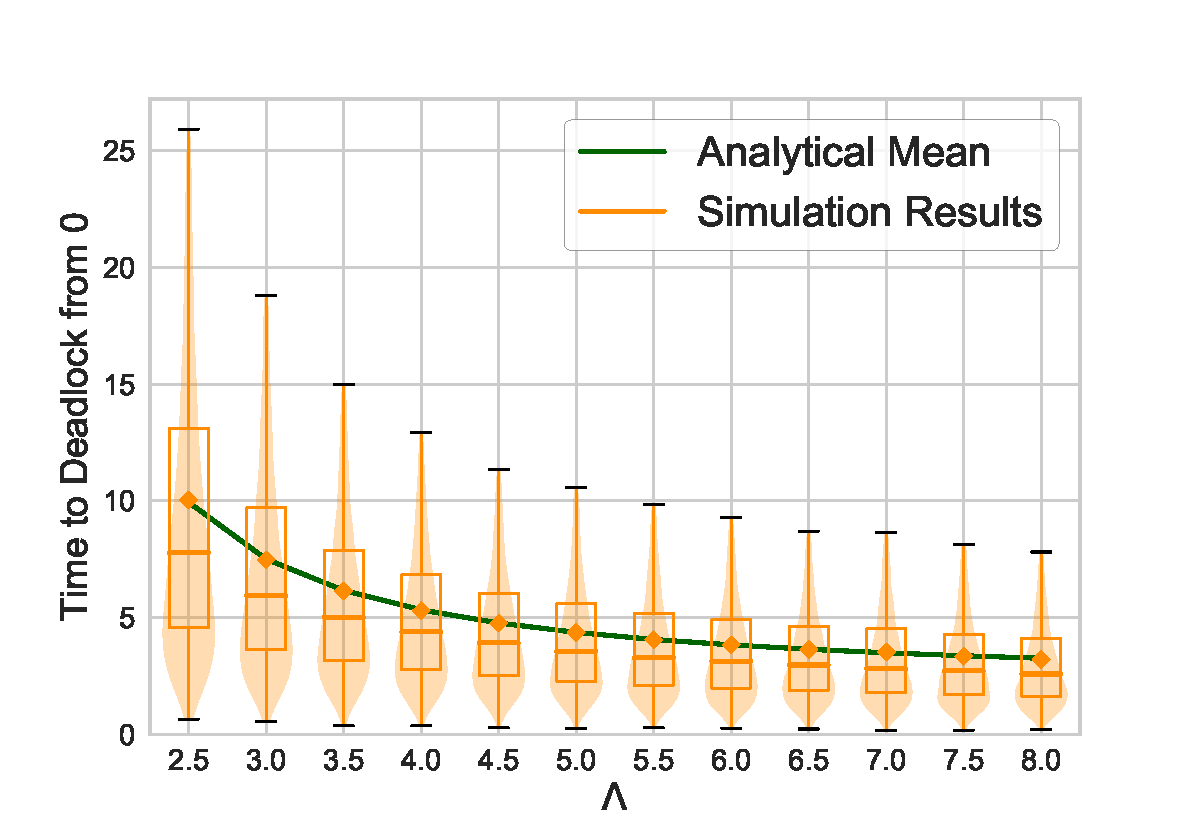
\includegraphics[width=\textwidth]{images/1Nms_varyL}
    \caption{Varying $\Lambda$}
    \label{fig:1Nms_L}
  \end{subfigure}
  \begin{subfigure}[b]{0.48\textwidth}
    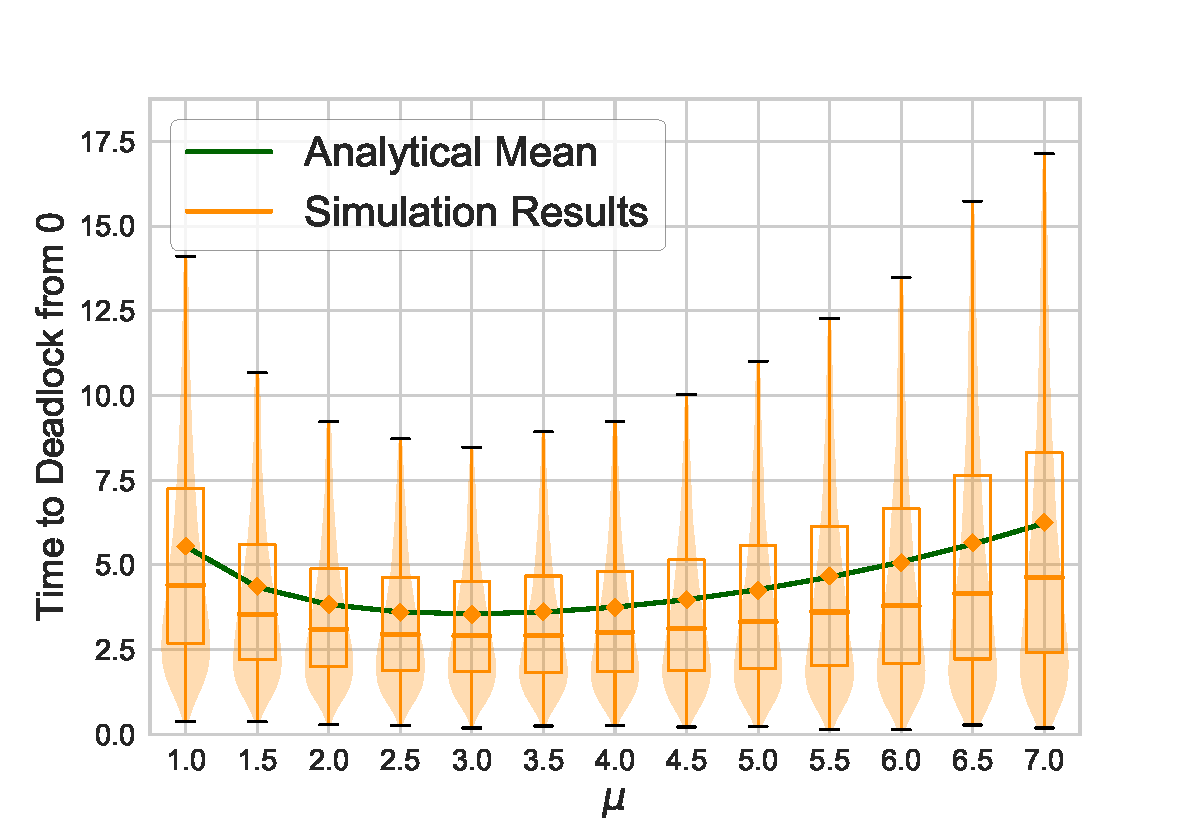
\includegraphics[width=\textwidth]{images/1Nms_varymu}
    \caption{Varying $\mu$}
    \label{fig:1Nms_mu}
  \end{subfigure}\\
  \begin{subfigure}[b]{0.48\textwidth}
    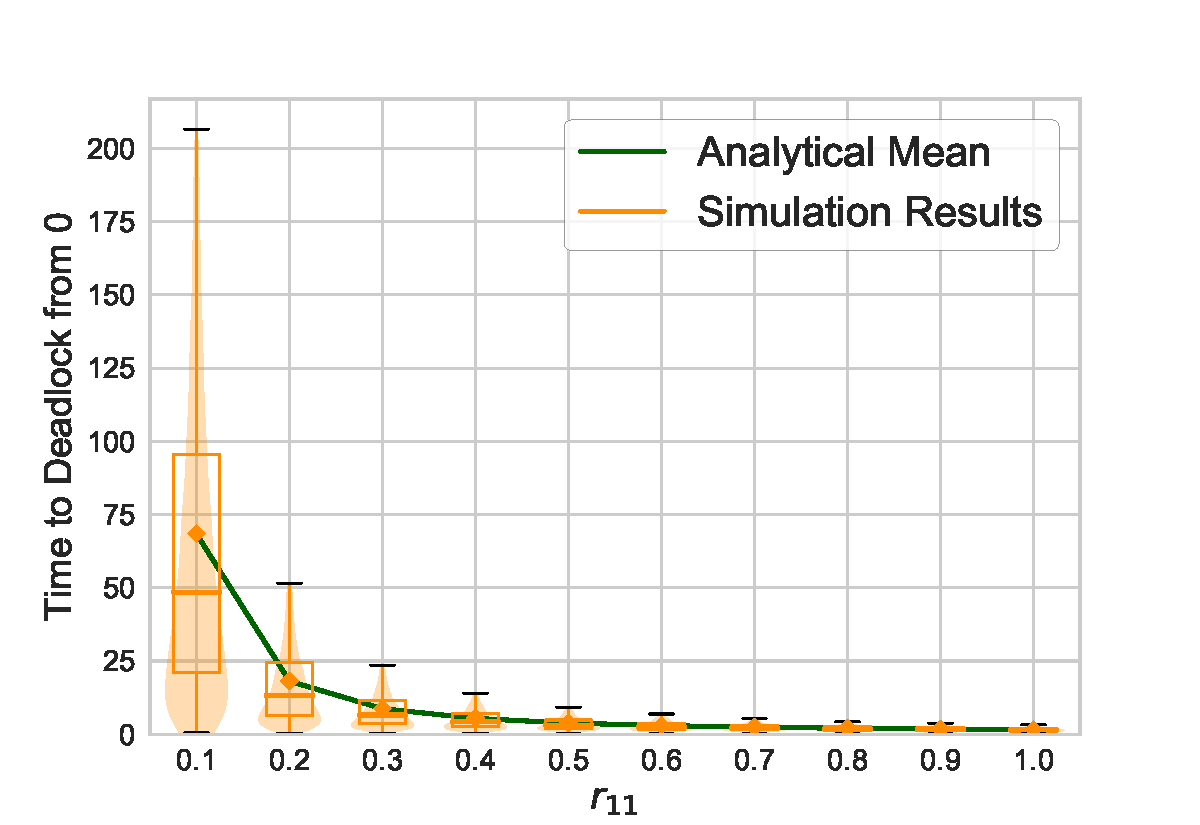
\includegraphics[width=\textwidth]{images/1Nms_varyr11}
    \caption{Varying $r_{11}$}
    \label{fig:1Nms_r11}
  \end{subfigure}
  \begin{subfigure}[b]{0.48\textwidth}
    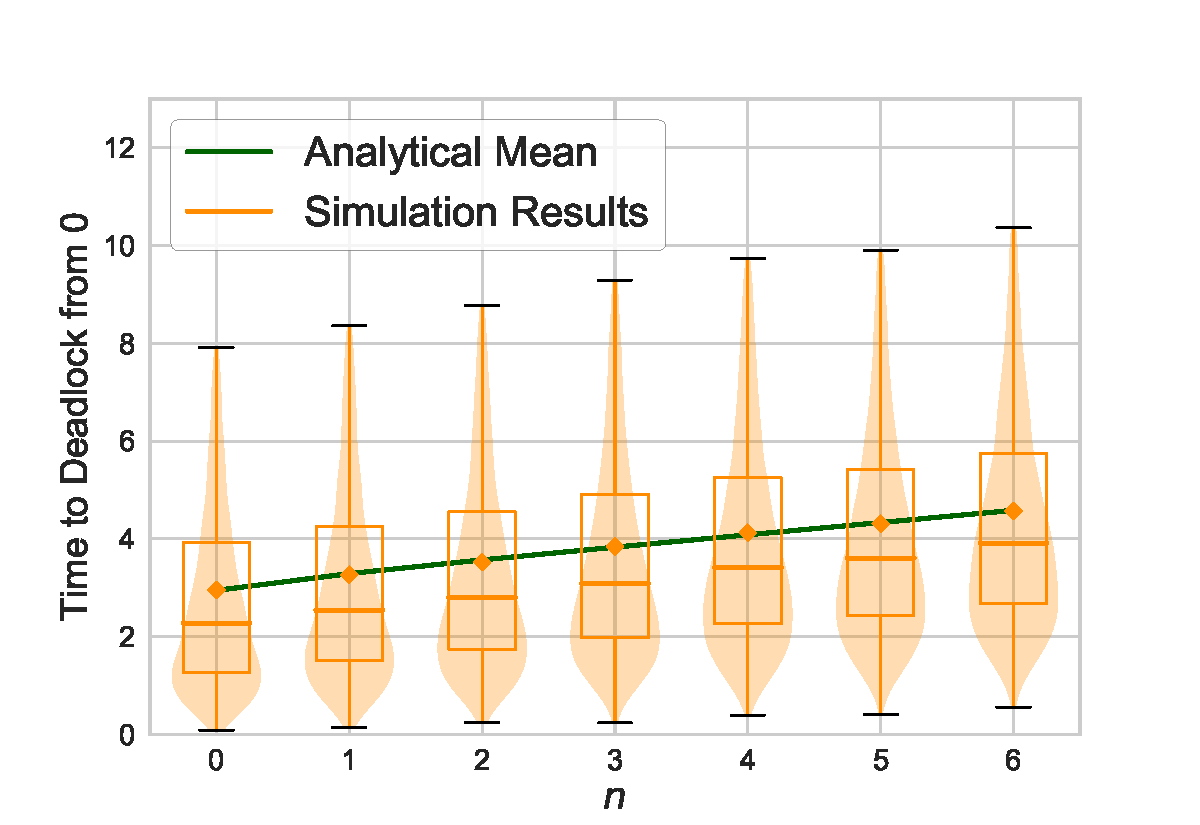
\includegraphics[width=\textwidth]{images/1Nms_varyn}
    \caption{Varying $n$}
    \label{fig:1Nms_n}
  \end{subfigure}\\
  \begin{subfigure}[b]{0.48\textwidth}
    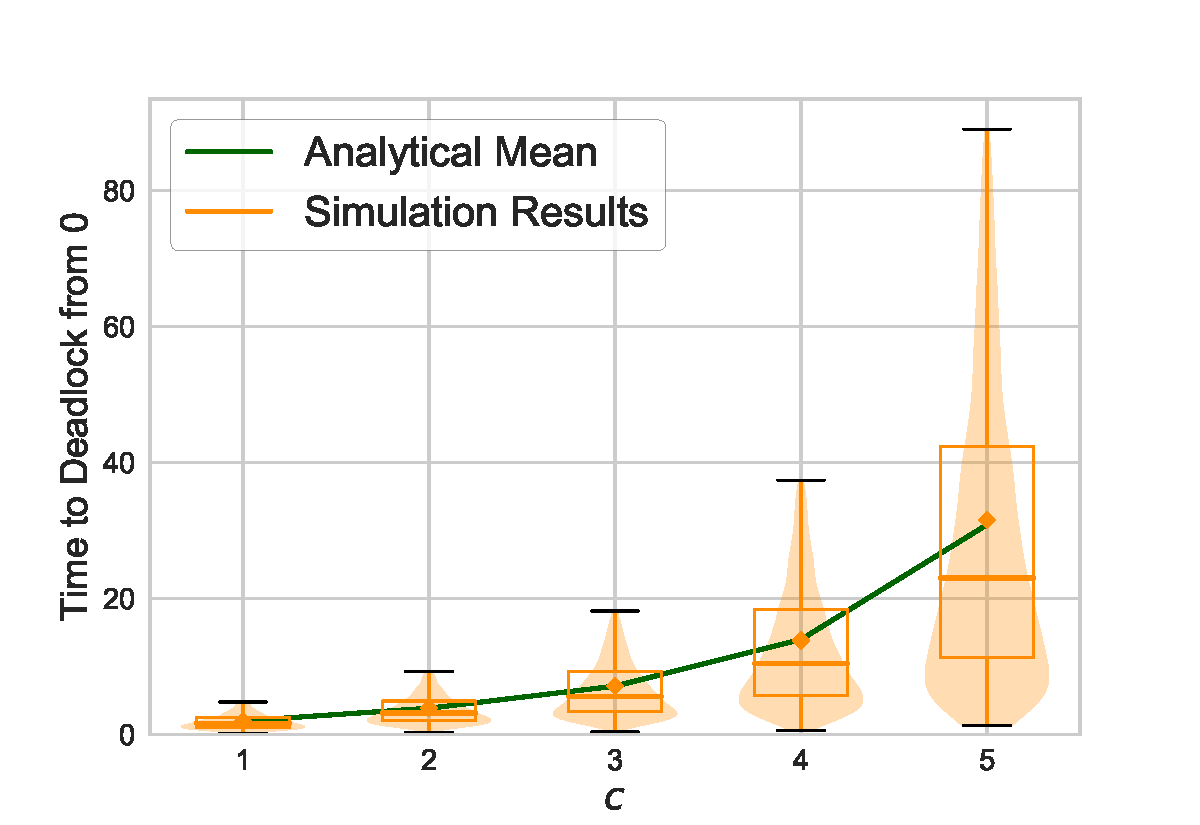
\includegraphics[width=\textwidth]{images/1Nms_varyc}
    \caption{Varying $c$}
    \label{fig:1Nms_c}
  \end{subfigure}
  \end{center}
  \caption{Time to deadlock in multi-server $\Omega_1$, analytical \&
  simulation results (10,000 repetitions).}
  \label{fig:timestodeadlock1nodemultiserver}
\end{figure}

It can be seen that increasing the arrival rate $\Lambda$ and the routing
probability $r_{11}$ results in reaching deadlock faster.
This is intuitive as increasing these parameters results in the queue filling
up quicker.
Increasing the queueing capacity $n$ results in reaching deadlock later.
Again this is intuitive, as increasing the queueing capacity allows more
customers in the system before becoming deadlocked.

Increasing the amount of servers has a similar effect to increasing the
queueing capacity, there are now more transient states to go through before
reaching the deadlocked state.
Varying the amount of servers has a greater effect on the time to deadlock
however, as any states in which customers are blocked, $i \in [n+c+1, n+2c]$,
can jump back to state $i=n+c-1$ simply with a service where the customer
doesn't rejoin the queue.
Increasing the amount of servers also increases the rate at which $i$ are
reduced for most states, but doesn't affect the rates at which $i$ is
increased.

The behaviour as the service rate $\mu$ varies is not monotonic, as the
service rate contributes towards both moving customers from the system and
allowing customers to rejoin the queue, causing blockages and deadlock.
This behaviour is described in the following remark.\\

\begin{remark}\label{rem:oneminima}
The function $\omega_1(\mu)$ that describes the expected time to deadlock of
an $\Omega_1$ system as the service rate $\mu$ varies, and all other
parameters are fixed, has one critical point and is a local minimum for
$\mu \in (0, \infty)$.
\end{remark}

The behaviour of $\omega_1(\mu)$ can be interpreted as follows:
\begin{itemize}
\item At $\lim_{\mu \to 0} \omega_1 (\mu)$ there is infinite service time,
and so infinite time until deadlock.
\item At $\lim_{\mu \to \infty} \omega_1 (\mu)$ there is zero service time,
the queue can never fill up, and so infinite time to deadlock.
\item At low service rates below a certain threshold $\hat{\mu}$, the arrival
rate is relatively large compared to the service rate, and we can assume a
saturated system.
At this point services where a customer exits the system does not have much of
an effect, as we can assume another arrival immediately.
However services where a customer wishes to rejoin the queue results in a
blockage as the system is saturated.
Therefore, increasing the service rate here increases the chance of a
blockage, and so the chance of deadlock.
\item Above $\hat{\mu}$ the service rate is large enough that we cannot assume
a saturated system, and so services where the customer exits the system does
have an affect on the number of customers in the system.
Thus increasing the service rate removes people from the system, and as such
there is less chance of getting blocked and reaching deadlock.
\end{itemize}

The following remark identifies the maximum of $\omega_1(\mu)$ on a closed
interval.\\

\begin{remark}\label{rem:findmaximum}
$\arg\max_{\mu \in [a, b]} \omega_1(\mu) \in \{a, b\}$.

From the closed interval method of finding absolute maximum \cite{tan09}, the
absolute maximum of $\omega_1(\mu)$ on the closed interval $[a, b]$ is either
the critical points in $(a, b)$, $a$ or $b$.
The only possible critical point in $(a, b)$ is $\hat{\mu}$, and is a local
minimum (from Remark~\ref{rem:oneminima}), and so
$\omega_1(\hat{\mu}) \leq \omega_1(a)$ and
$\omega_1(\hat{\mu}) \leq \omega_1(b)$.
Therefore $\omega_1(\mu)$ obtains its maximum at either $a$ or $b$.
\end{remark}


\subsection{Two Node Multi-Server without Self-Loops}\label{sec:2nodeMS}

Consider the open two node multi-server restricted queueing network shown in
Figure~\ref{fig:queueingnetwork_2nodemulti}.
This shows two \(M/M/c_i/n_i\) queues, with service rates $\mu_i$ and external
arrival rates $\Lambda_i$.
All routing possibilities $r_{ij}$ are possible except self-loops $r_{ii}$ for
each node $i$.

Let this system be denoted by $\Omega_2$ with parameter set $(\Lambda_1$,
$\Lambda_2$, $\mu_1$, $\mu_2$, $c_1$, $c_2$, $n_1$, $n_2$, $r_{12}$, $r_{21})$,
and the time to deadlock of this system be denoted by $\omega_2$.

\begin{figure}[!htbp]
  \begin{center}
  \includestandalone[width=0.75\textwidth]{images/2nodemultiserver}
  \end{center}
  \caption{An open two node multi-server restricted queueing network.}
  \label{fig:queueingnetwork_2nodemulti}
\end{figure}

The state space is given by:
        \[S = \{(i,j)\in\mathbb{N}^{(n_1+c_1+c_2)\times (n_2+c_2+c_1)} \nonscript\; | \nonscript\; i \leq n_1+c_1+j, \nonscript\; j \leq n_2+c_2+i\}\]
where $i$ denotes the number of individuals at Node 1 plus the number of
individuals blocked waiting to enter Node 1, and $j$ denotes the number of
individuals at Node 2 plus the number of individuals blocked waiting to enter
Node 2.
For example, $(i, j) = (n_1+c_1+2, n_2+c_2+1)$ denotes a full system,
$n_1+c_1$ individuals at Node 1, two of whom are blocked waiting to enter
Node 2; $n_2+c_2$ individuals at Node 2, one of whom is blocked waiting to
enter Node 1.
The state $(i, j) = (n_1+c_1+c_2, n_2+c_2+c_1)$ denotes the deadlocked state.

The Markov chain is shown in Figure~\ref{fig:2nodeMCms}.

\begin{figure}[!htbp]
    \includestandalone[width=\textwidth]{images/MC2nodemultiserv_bw}
    \caption{Diagrammatic representation of the Markov chain for a
    multi-server $\Omega_2$ system with $n_1=1$, $n_2=c_1=c_2=2$.
    The deadlocked state is $(5,6)$.}
    \label{fig:2nodeMCms}
\end{figure}

Define $\delta = (i_2, j_2) - (i_1, j_1)$, $b_1 = \max(0, i_1-n_1-c_1)$,
$b_2 = \max(0, i_2-n_2-c_2)$, $s_1 = \min(i_1, c_1)-b_2$ and
$s_2 = \min(i_2, c_2)-b_1$ for all $(i_k, j_k) \in S$.
Then the transitions $q_{(i_1, j_1),(i_2, j_2)}$ are given by
Table~\ref{tab:transitionsmultierv}.


\begin{table}
\begin{center}
\resizebox{\textwidth}{!}{
\begin{tabular}{ l l l l }
  \toprule
  & $j_1 < n_2 + c_2$ & $j_1 = n_2 + c_2$ & $ j_1 > n_2 + c_2$ \\
  \midrule
  $i_1 < n_1 + c_1$ & \begin{tabular}{ l } $\Lambda_1$ if $\delta = (1, 0)$ \\ $\Lambda_2$ if $\delta = (0, 1)$ \\ $r_{12}s_1\mu_1$ if $\delta = (-1, 1)$ \\ $r_{21}s_2\mu_2$ if $\delta = (1, -1)$ \\ $(1-r_{12})s_1\mu_1$ if $\delta = (-1, 0)$ \\ $(1-r_{21})s_2\mu_2$ if $\delta = (0, -1)$ \end{tabular} & \begin{tabular}{ l } $\Lambda_1$ if $\delta = (1, 0)$ \\ $r_{12}s_1\mu_1$ if $\delta = (0, 1)$ \\ $r_{21}s_2\mu_2$ if $\delta = (1, -1)$ \\ $(1-r_{12})s_1\mu_1$ if $\delta = (-1, 0)$ \\ $(1-r_{21})s_2\mu_2$ if $\delta = (0, -1)$ \end{tabular} & \begin{tabular}{ l } $\Lambda_1$ if $\delta = (1, 0)$ \\ $r_{12}s_1\mu_1$ if $\delta = (0, 1)$ \\ $r_{21}s_2\mu_2$ if $\delta = (0, -1)$ \\ $(1-r_{12})s_1\mu_1$ if $\delta = (-1, 0)$ \\ $(1-r_{21})s_2\mu_2$ if $\delta = (-1, -1)$ \end{tabular} \\
  \midrule
  $i_1 = n_1 + c_1$ & \begin{tabular}{ l } $\Lambda_2$ if $\delta = (0, 1)$ \\ $r_{12}s_1\mu_1$ if $\delta = (-1, 1)$ \\ $r_{21}s_2\mu_2$ if $\delta = (1, 0)$ \\ $(1-r_{12})s_1\mu_1$ if $\delta = (-1, 0)$ \\ $(1-r_{21})s_2\mu_2$ if $\delta = (0, -1)$ \end{tabular} & \begin{tabular}{ l } $r_{12}s_1\mu_1$ if $\delta = (0, 1)$ \\ $r_{21}s_2\mu_2$ if $\delta = (1, 0)$ \\ $(1-r_{12})s_1\mu_1$ if $\delta = (-1, 0)$ \\ $(1-r_{21})s_2\mu_2$ if $\delta = (0, -1)$ \end{tabular} & \begin{tabular}{ l } $r_{12}s_1\mu_1$ if $\delta = (0, 1)$ \\ $r_{21}s_2\mu_2$ if $\delta = (1, 0)$ \\ $(1-r_{12})s_1\mu_1$ if $\delta = (-1, 0)$ \\ $(1-r_{21})s_2\mu_2$ if $\delta = (-1, -1)$ \end{tabular} \\
  \midrule
  $i_1 > n_1 + c_1$ & \begin{tabular}{ l } $\Lambda_2$ if $\delta = (0, 1)$ \\ $r_{12}s_1\mu_1$ if $\delta = (-1, 0)$ \\ $r_{21}s_2\mu_2$ if $\delta = (1, 0)$ \\ $(1-r_{12})s_1\mu_1$ if $\delta = (-1, -1)$ \\ $(1-r_{21})s_2\mu_2$ if $\delta = (0, -1)$ \end{tabular} & \begin{tabular}{ l } $r_{12}s_1\mu_1$ if $\delta = (0, 1)$ \\ $r_{21}s_2\mu_2$ if $\delta = (1, 0)$ \\ $(1-r_{12})s_1\mu_1$ if $\delta = (-1, -1)$ \\ $(1-r_{21})s_2\mu_2$ if $\delta = (0, -1)$ \end{tabular} & \begin{tabular}{ l } $r_{12}s_1\mu_1$ if $\delta = (0, 1)$ \\ $r_{21}s_2\mu_2$ if $\delta = (1, 0)$ \\ $(1-r_{12})s_1\mu_1$ if $\delta = (-\min(b_1+1,b_2+1), -\min(b_1,b_2+1))$ \\ $(1-r_{21})s_2\mu_2$ if $\delta = (-\min(b_1+1,b_2), -\min(b_1+1,b_2+1))$ \end{tabular} \\
  \bottomrule
\end{tabular}
}
\caption{Table of transitions $q_{(i_1, j_1),(i_2, j_2)}$ for a multi-server
two node network.}
\label{tab:transitionsmultierv}
\end{center}
\end{table}


The values $b_1$ and $b_2$ correspond to the number of people blocked to
Node 1 and Node 2 respectively.
The values $s_1$ and $s_2$ correspond to the amount of people currently in
service at Node 1 and Node 2 respectively.

Figure~\ref{fig:timestodeadlock2nodemultiserver} shows the effect of varying
the parameters of the above Markov model.
Base parameters of $\Lambda_1 = 9$, $\Lambda_2 = 7.5$, $n_1 = 2$, $n_2 = 1$,
$\mu_1 = 5.5$, $\mu_2 = 6.5$, $r_{12} = 0.7$, $r_{21} = 0.6$, $c_1 = 2$ and
$c_2 = 2$ were used.

\begin{figure}[!htbp]
  \begin{center}
  \begin{subfigure}[b]{0.48\textwidth}
    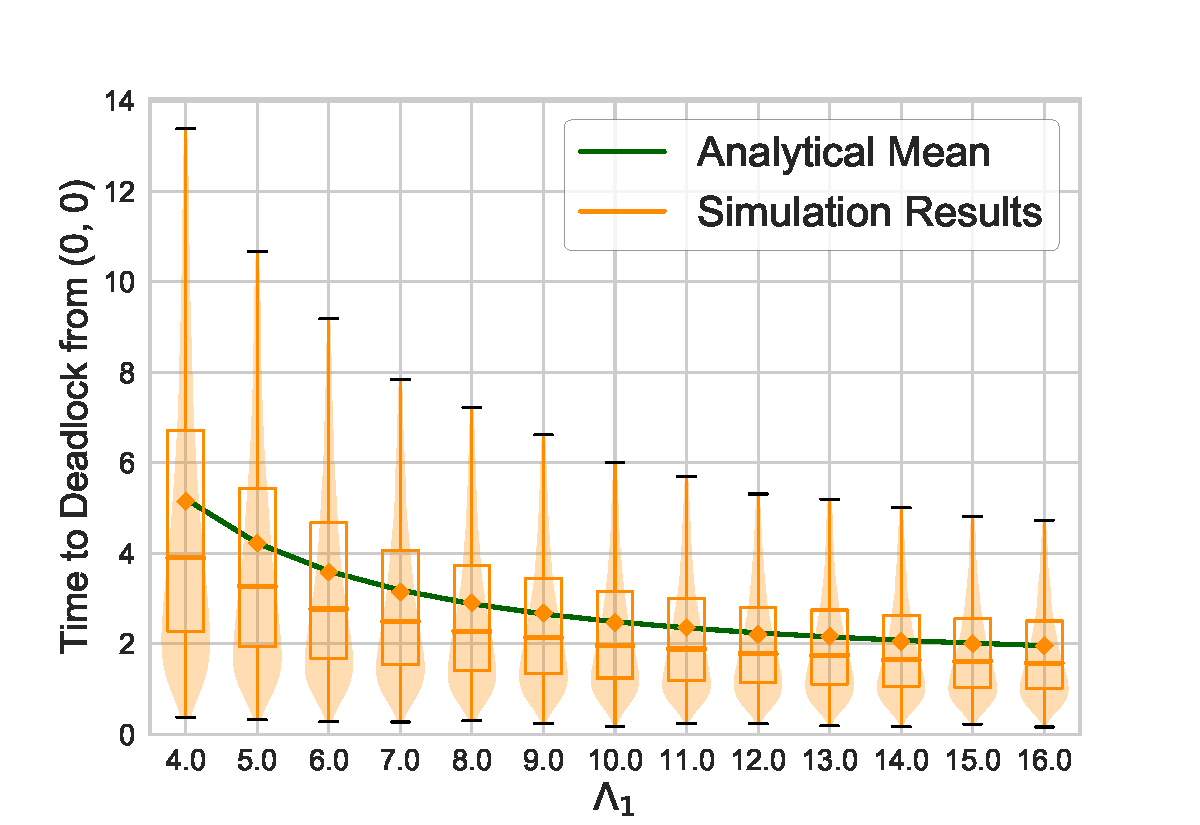
\includegraphics[width=\textwidth]{images/2Nms_varyL1}
    \caption{Varying $\Lambda_1$}
    \label{fig:2Nms_L}
  \end{subfigure}
  \begin{subfigure}[b]{0.48\textwidth}
    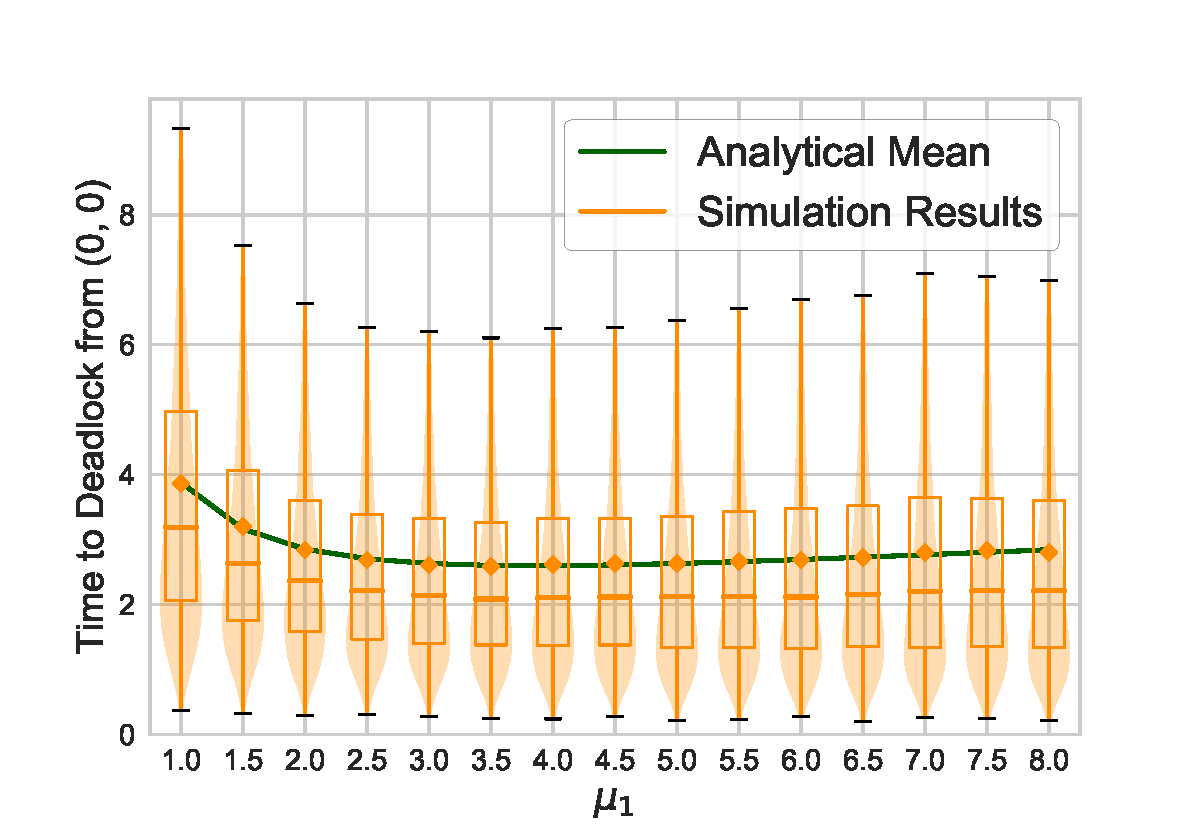
\includegraphics[width=\textwidth]{images/2Nms_varymu1}
    \caption{Varying $\mu_1$}
    \label{fig:2Nms_mu}
  \end{subfigure}\\
  \begin{subfigure}[b]{0.48\textwidth}
    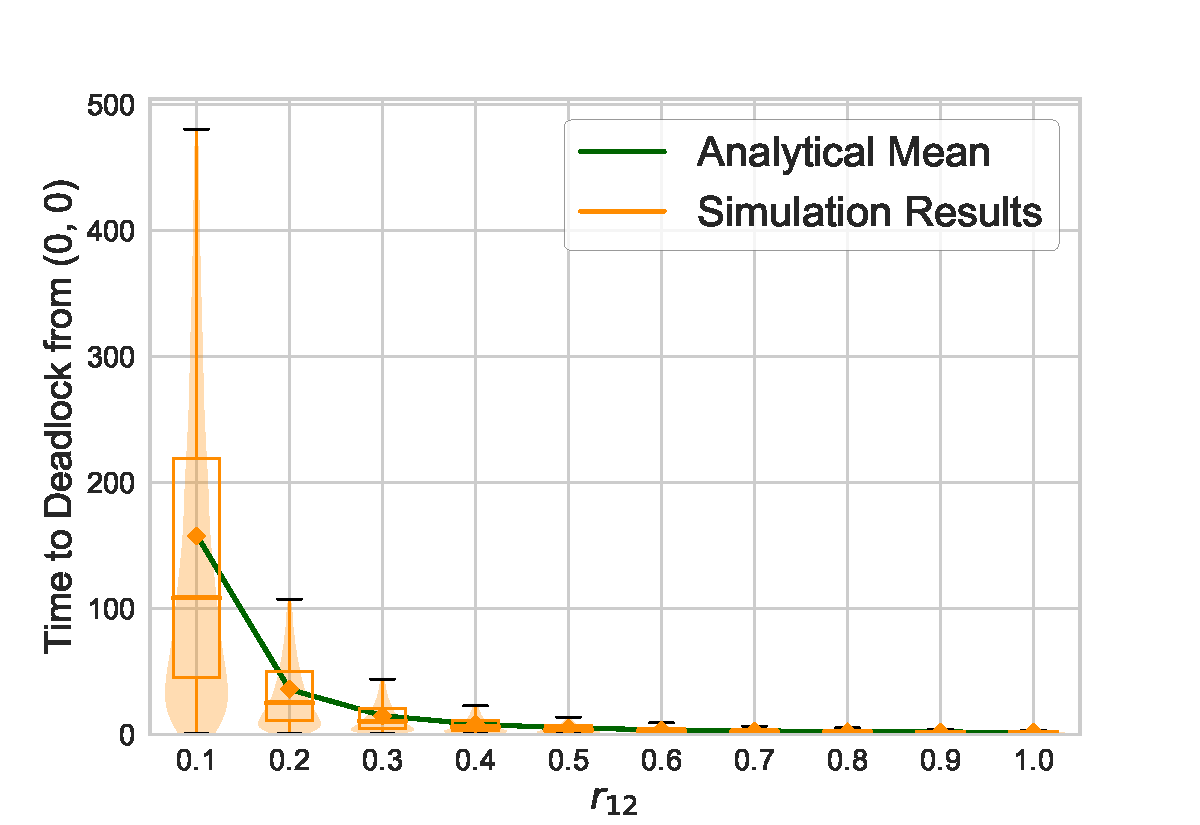
\includegraphics[width=\textwidth]{images/2Nms_varyr12}
    \caption{Varying $r_{12}$}
    \label{fig:2Nms_r11}
  \end{subfigure}
  \begin{subfigure}[b]{0.48\textwidth}
    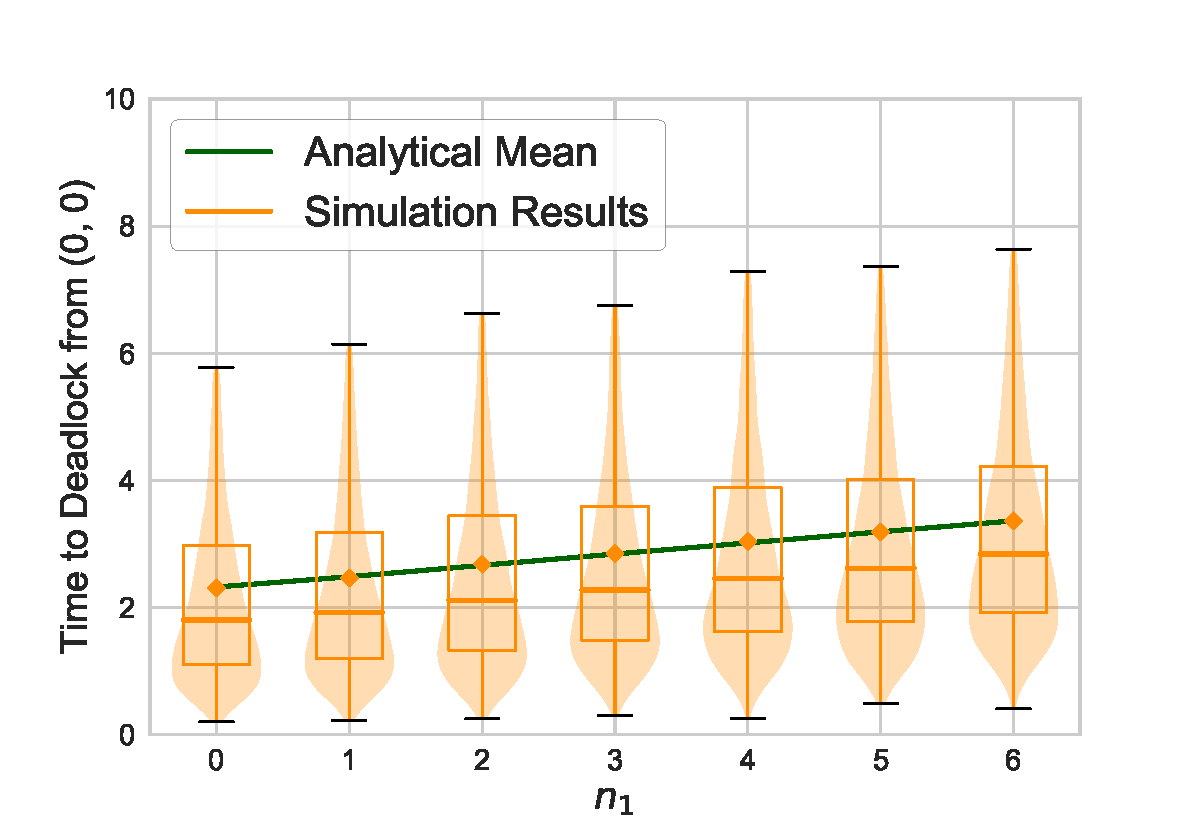
\includegraphics[width=\textwidth]{images/2Nms_varyn1}
    \caption{Varying $n_1$}
    \label{fig:2Nms_n}
  \end{subfigure}\\
  \begin{subfigure}[b]{0.48\textwidth}
    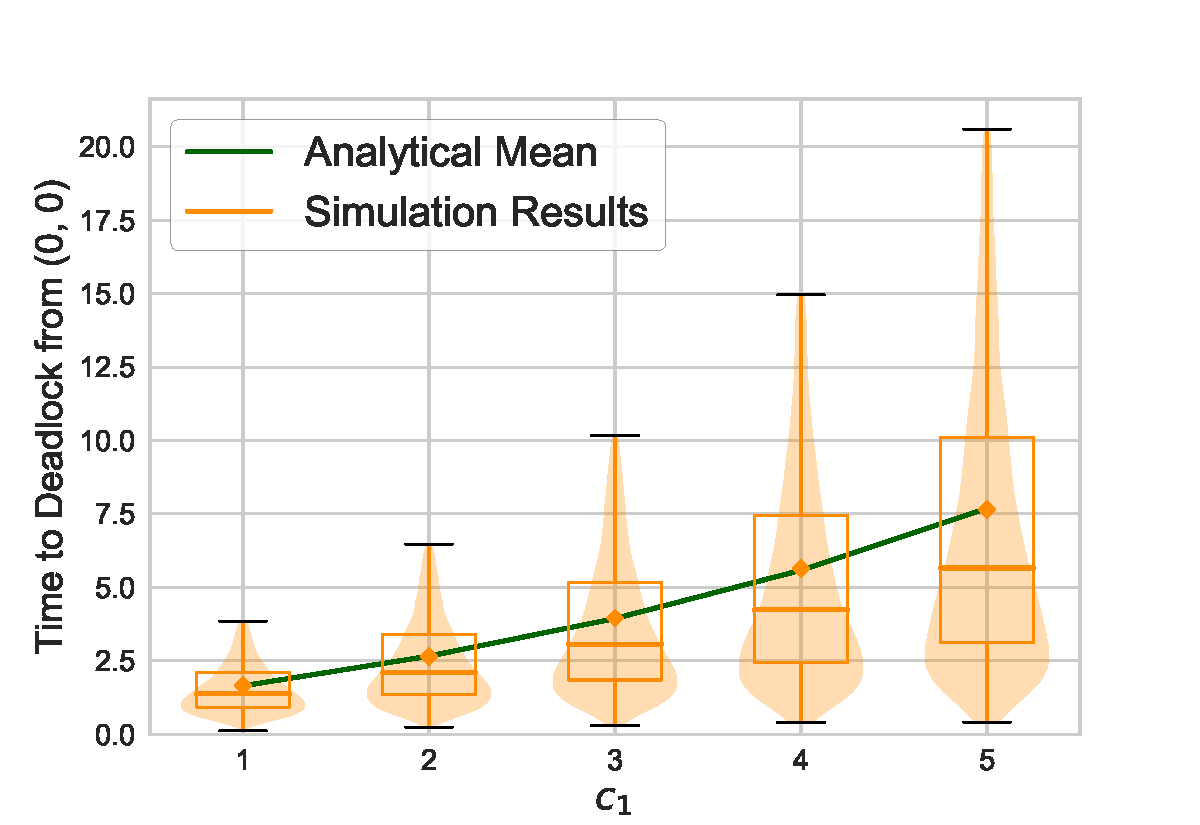
\includegraphics[width=\textwidth]{images/2Nms_varyc1}
    \caption{Varying $c_1$}
    \label{fig:2Nms_c}
  \end{subfigure}
  \end{center}
  \caption{Time to deadlock in multi-server $\Omega_2$, analytical \&
  simulation results (10,000 repetitions).}
  \label{fig:timestodeadlock2nodemultiserver}
\end{figure}


\subsection{Two Node Single-Server with Self-Loops}\label{sec:2nodeselfloops}

Consider the open two node single-server restricted queueing network shown in
Figure~\ref{fig:queueingnetwork_2nodesfeedback}.
This shows two \(M/M/1/n_i\) queues with service rates $\mu_i$  and external
arrival rates $\Lambda_i$.
All routes are possible, where the routing probability from node $i$ to node
$j$ is denoted by $r_{ij}$.

Let this system be denoted by $\Omega$ with parameter set $(\Lambda_1$,
$\Lambda_2$, $\mu_1$, $\mu_2$, $n_1$, $n_2$, $r_{11}$, $r_{12}$, $r_{21}$,
$r_{22})$.

\begin{figure}[!htbp]
  \begin{center}
  \includestandalone[width=0.75\textwidth]{images/2nodefeedbackexample}
  \end{center}
  \caption{An open two node single-server restricted queueing network.}
  \label{fig:queueingnetwork_2nodesfeedback}
\end{figure}

The state space is given by:
    \[S = \{(i,j)\in\mathbb{N}^{(n_1+2)\times (n_2+2)} \nonscript\; | \nonscript\; 0 \leq i + j \leq n_1 + n_2 + 2
    \}\cup\{(-1), (-2), (-3)\}\]

    where \(i\) denotes the number of individuals:
        \begin{itemize}
            \item In service or waiting at the first node.
            \item Occupying a server but having finished service at the
                second node waiting to join the first.
        \end{itemize}
    where \(j\) denotes the number of individuals:
        \begin{itemize}
            \item In service or waiting at the second node.
            \item Occupying a server but having finished service at the
                first node waiting to join the second.
        \end{itemize}
    and the state $(-3)$ denotes the deadlocked state caused by both nodes;
    $(-1)$ denotes the deadlocked state caused by the first node only; and
    $(-2)$ denotes the deadlocked state caused by the second node only.

Define $\delta = (i_2, j_2) - (i_1, j_1)$ for all $(i_k, j_k) \in S$.
The transitions are given by Equations~\ref{eqn:2nssfA}, \ref{equ:todeadlock2},
\ref{equ:todeadlock3} and \ref{eqn:2nssfB}.

\begin{equation}\label{eqn:2nssfA}
  q_{(i_1, j_1),(i_2, j_2)} = \left\{
  \begin{array}{rr}
    \left. \begin{array}{rr}
      \Lambda_1 & \text{if } i_1 < n_1 + 1 \\
      0 & \text{otherwise}
    \end{array} \right\} & \text{if } \delta = (1, 0) \\
    \left. \begin{array}{rr}
      \Lambda_2 & \text{if } j_1 < n_2 + 1 \\
      0 & \text{otherwise}
    \end{array} \right\} & \text{if } \delta = (0, 1) \\
    \left. \begin{array}{rr}
      (1 - r_{11} - r_{12})\mu_1 & \text{if } j_1 < n_2 + 2 \\
      0 & \text{otherwise}
    \end{array} \right\} & \text{if } \delta = (-1, 0) \\
    \left. \begin{array}{rr}
      (1 - r_{21} - r_{22})\mu_2 & \text{if } i_1 < n_1 + 2 \\
      0 & \text{otherwise}
    \end{array} \right\} & \text{if } \delta = (0, -1) \\
    \left. \begin{array}{rr}
      r_{12}\mu_1 & \text{if } j_1 < n_2 + 2 \text{ and } (i_1, j_1) \neq (n_1 + 2, n_2) \\
      0 & \text{otherwise}
    \end{array} \right\} & \text{if } \delta = (-1, 1) \\
    \left. \begin{array}{rr}
      r_{21}\mu_2 & \text{if } i_1 < n_1 + 2 \text{ and } (i_1, j_1) \neq (n_1, n_2 + 2) \\
      0 & \text{otherwise}
    \end{array} \right\} & \text{if } \delta = (1, -1) \\
    0 & \text{otherwise}
  \end{array} \right.
\end{equation}

\begin{equation}\label{equ:todeadlock2}
  q_{(i_1, j_1), (-1)} = \left\{
  \begin{array}{rr}
    r_{11}\mu_1 & \text{if } i > n_1 \text{ and } j < n_2 + 2 \\
    0 & \text{otherwise}
  \end{array}
  \right.
\end{equation}

\begin{equation}\label{equ:todeadlock3}
  q_{(i_1, j_1), (-2)} = \left\{
  \begin{array}{rr}
    r_{22}\mu_2 & \text{if } j > n_2 \text{ and } i < n_1 + 2 \\
    0 & \text{otherwise}
  \end{array}
  \right.
\end{equation}

\begin{equation}\label{eqn:2nssfB}
  q_{(i_1, j_1), (-3)} = \left\{
  \begin{array}{rr}
    r_{21}\mu_2 & \text{if } (i, j) = (n_1, n_2 + 2) \\
    r_{12}\mu_1 & \text{if } (i, j) = (n_1 + 2, n_2) \\
    0 & \text{otherwise}
  \end{array}
  \right.
\end{equation}

\begin{align}
  q_{-1, s} = 0 \\
  q_{-2, s} = 0 \\
  q_{-3, s} = 0
\end{align}

Note that there are now three different deadlock states, thus two more ways to
reach deadlock, Equation~\ref{equ:todeadlock2} and Equation~\ref{equ:todeadlock3}.

For $n_1 = 1$ and $n_2 = 2$, the resulting Markov chain is shown in
Figure~\ref{fig:2nodeMCfeedback}.

\begin{figure}[!htbp]
    \begin{center}
    \includestandalone[width=\textwidth]{images/markov_chain_feedback_bw}
    \end{center}
    \caption{Diagrammatic representation of the Markov chain for $\Omega$ with
    $n_1=1$ and $n_2=2$.}
    \label{fig:2nodeMCfeedback}
\end{figure}

Figure~\ref{fig:timestodeadlockfeedback} shows the effect on the time to
deadlock of varying the parameters of the above Markov model.
Base parameters of $\Lambda_1 = 4$, $\Lambda_2 = 5$, $n_1 = 3$, $n_2 = 2$,
$\mu_1 = 10$, $\mu_2 = 8$, $r_{11} = 0.1$, $r_{12} = 0.25$, $r_{21} = 0.15$
and $r_{22} = 0.1$ are used.


\begin{figure}[!htbp]
\begin{center}
\begin{subfigure}[b]{0.48\textwidth}
  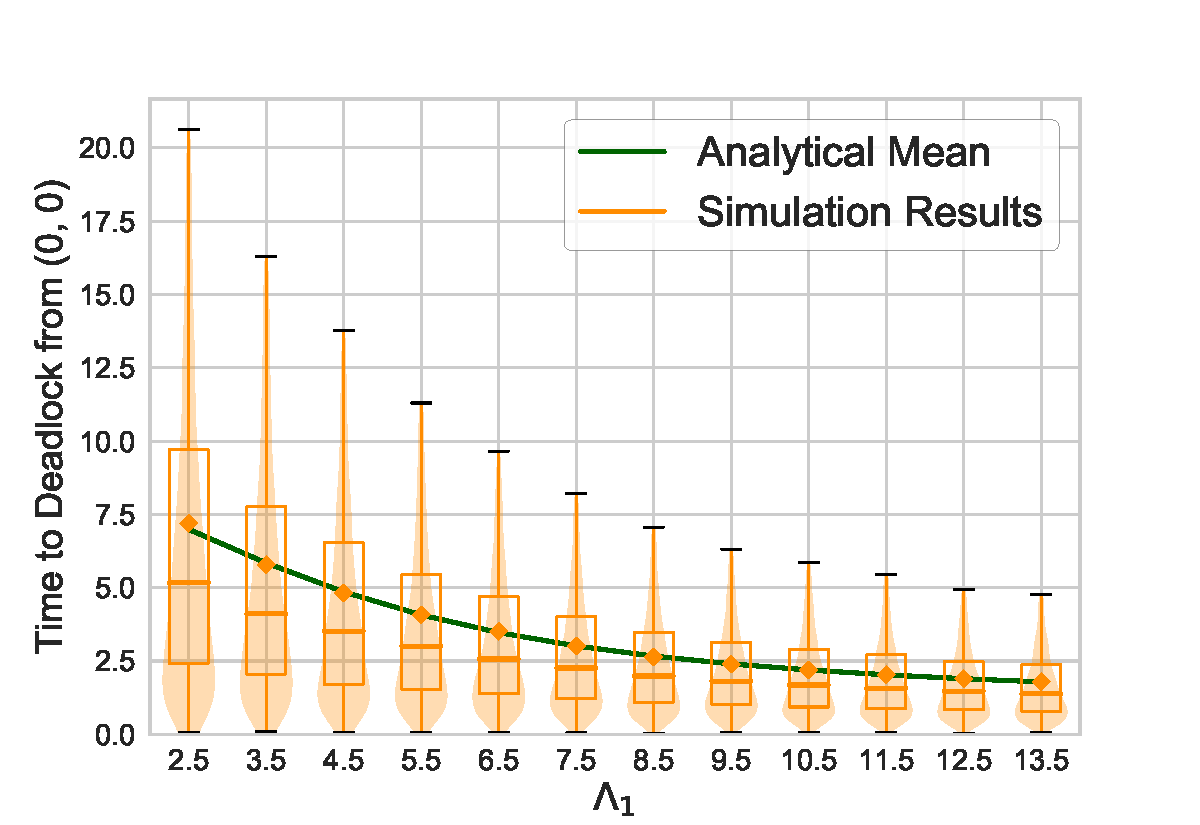
\includegraphics[width=\textwidth]{images/2Nmsfb_varyL1}
  \caption{Varying $\Lambda_1$}
  \label{fig:timestodeadlockfb_L1}
\end{subfigure}
\begin{subfigure}[b]{0.48\textwidth}
  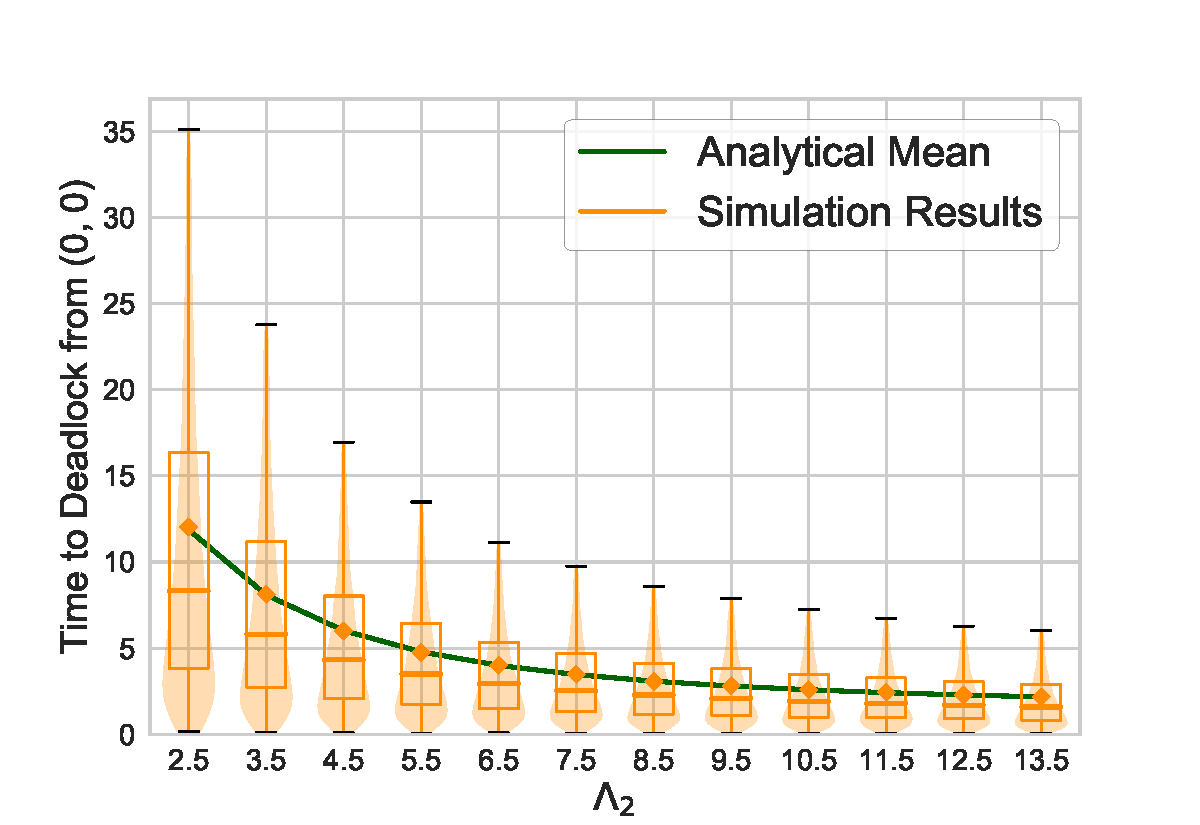
\includegraphics[width=\textwidth]{images/2Nmsfb_varyL2}
  \caption{Varying $\Lambda_2$}
  \label{fig:timestodeadlockfb_L2}
\end{subfigure}\\
\begin{subfigure}[b]{0.48\textwidth}
  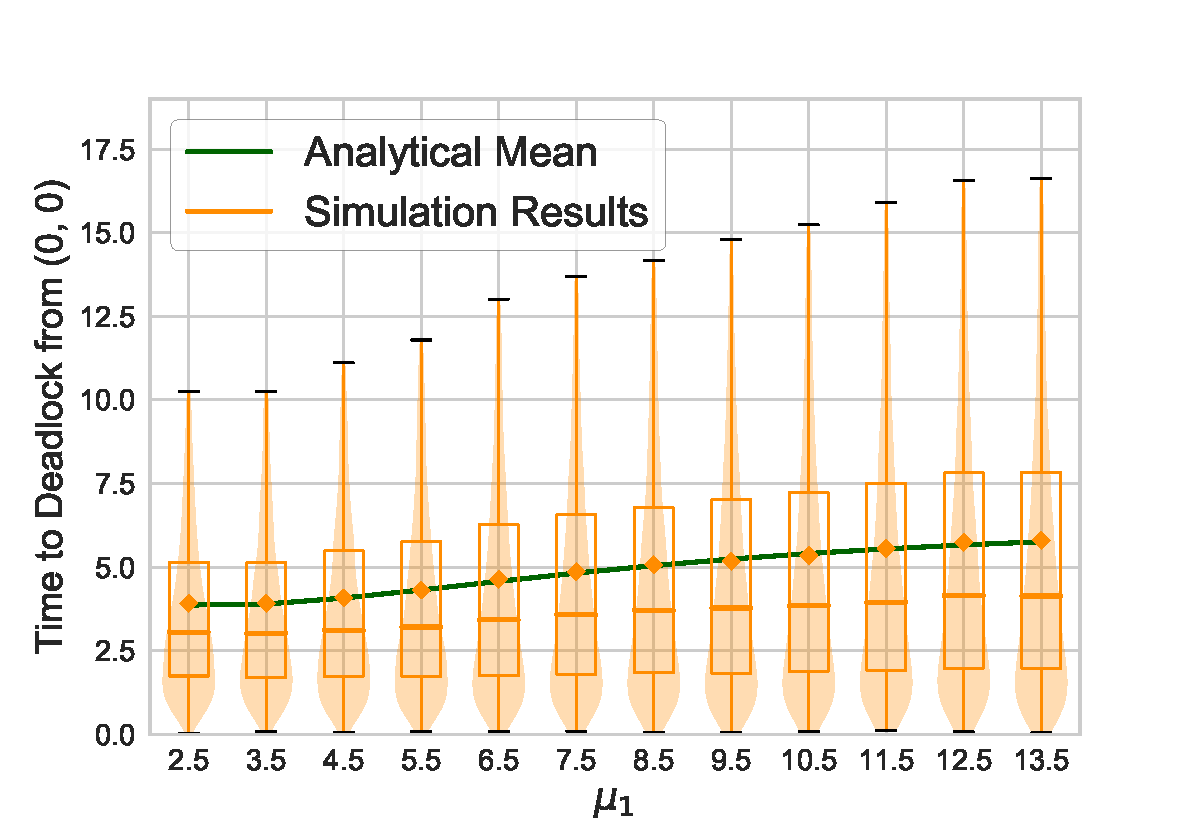
\includegraphics[width=\textwidth]{images/2Nmsfb_varymu1}
  \caption{Varying $\mu_1$}
  \label{fig:timestodeadlockfb_mu1}
\end{subfigure}
\begin{subfigure}[b]{0.48\textwidth}
  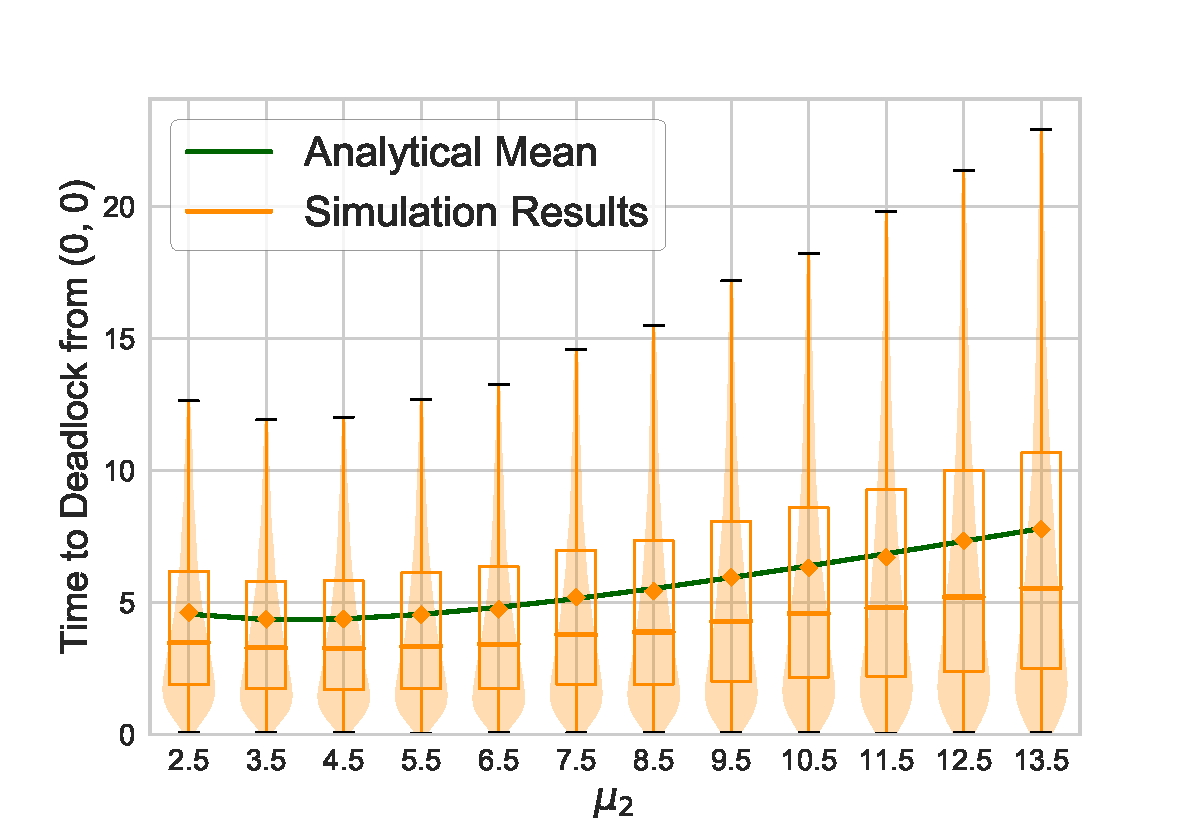
\includegraphics[width=\textwidth]{images/2Nmsfb_varymu2}
  \caption{Varying $\mu_2$}
  \label{fig:timestodeadlockfb_mu2}
\end{subfigure}\\
\begin{subfigure}[b]{0.48\textwidth}
  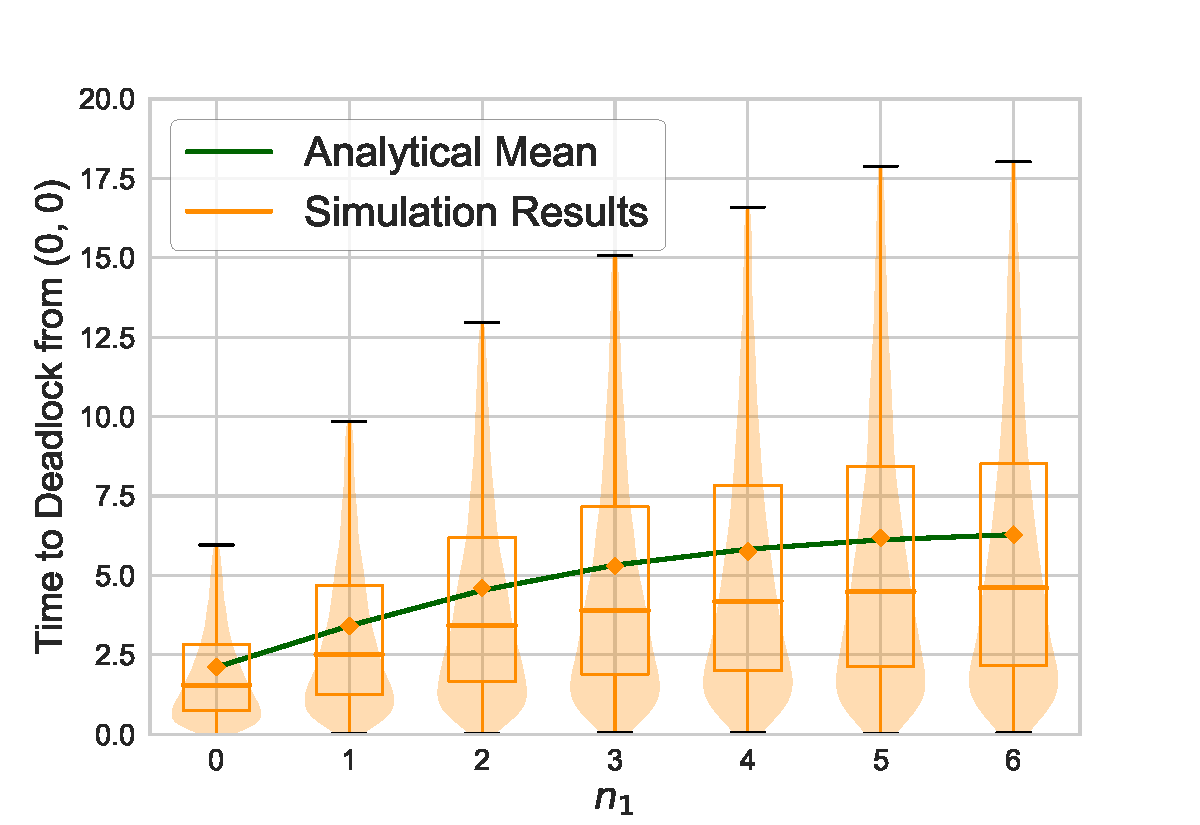
\includegraphics[width=\textwidth]{images/2Nmsfb_varyn1}
  \caption{Varying $n_1$}
  \label{fig:timestodeadlockfb_n1}
\end{subfigure}
\begin{subfigure}[b]{0.48\textwidth}
  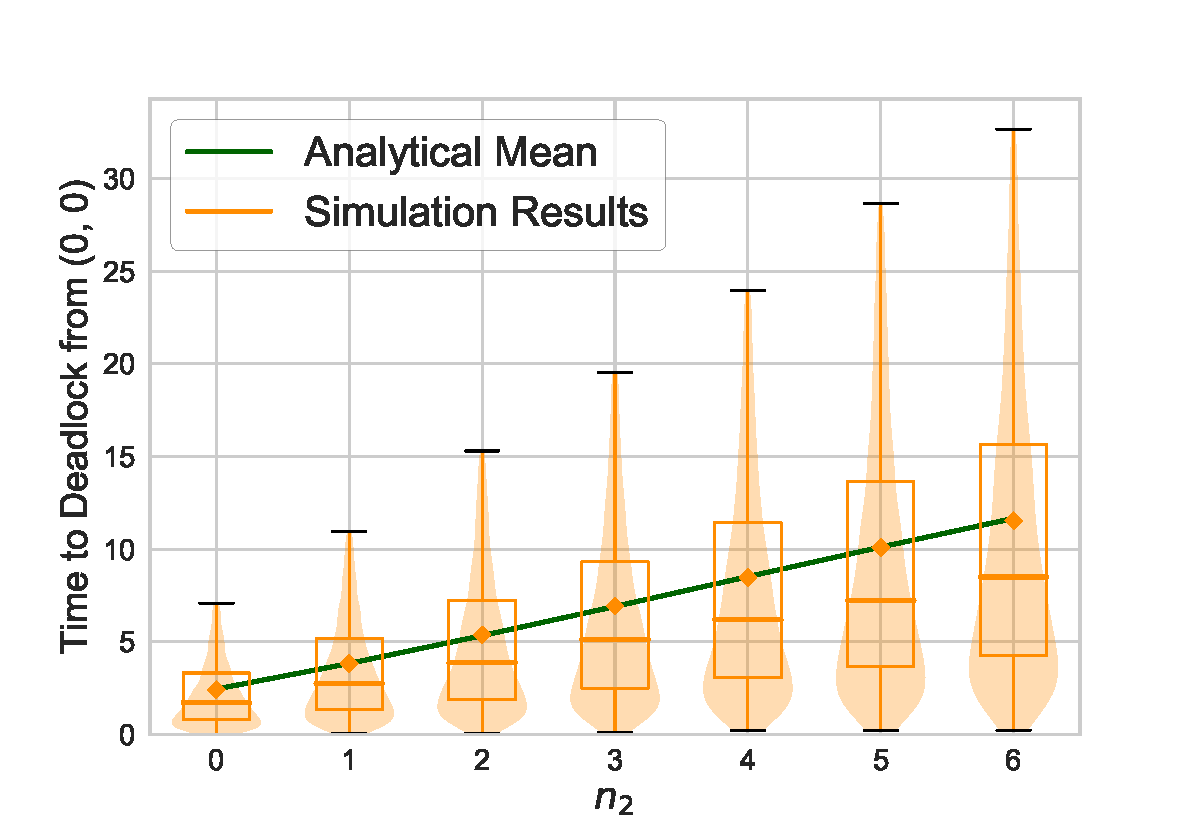
\includegraphics[width=\textwidth]{images/2Nmsfb_varyn2}
  \caption{Varying $n_2$}
  \label{fig:timestodeadlockfb_n2}
\end{subfigure}
\end{center}
\caption{Time to deadlock in $\Omega$, analytical \& simulation results
(10,000 repetitions).}
\label{fig:timestodeadlockfeedback}
\end{figure}



The next section derives a bound on the expected time to deadlock for the
single-server $\Omega$ system.


\section{A Bound on the Time to Deadlock}\label{sec:bound}

This section gives a bound on the expected time to deadlock of the $\Omega$
system.
After the bound is given, considerations on its tightness are given.
Let's define six deadlocking single-server queueing networks:

\begin{itemize}
  \item Define $\Omega_{1_1}^{\star}$ as an $\Omega_1$ system with the
  parameter set $(\Lambda_1$, $\mu_1$, $c_1=1$, $n_1$, $r_{11})$.\\
  Let its mean time to deadlock be denoted by $\omega_{1_1}^{\star}$.
  \item Define $\Omega_{1_1}^{\star\star}$ as an $\Omega_1$ system with the
  parameter set $(\Lambda_1$, $m_1$, $c_1=1$, $n_1$, $r_{11})$.\\
  Let its mean time to deadlock be denoted by $\omega_{1_1}^{\star\star}$.
  \item Define $\Omega_{1_2}^{\star}$ as an $\Omega_1$ system with the
  parameter set $(\Lambda_2$, $\mu_2$, $c_2=1$, $n_2$, $r_{22})$.\\
  Let its mean time to deadlock be denoted by $\omega_{1_2}^{\star}$.
  \item Define $\Omega_{1_2}^{\star\star}$ as an $\Omega_1$ system with the
  parameter set $(\Lambda_2$, $m_2$, $c_2=1$, $n_2$, $r_{22})$.\\
  Let its mean time to deadlock be denoted by $\omega_{1_2}^{\star\star}$.
  \item Define $\Omega_2$ with the parameter set $(\Lambda_1$, $\Lambda_2$,
  $\mu_1$, $\mu_2$, $c_1=1$, $c_2=1$, $n_1$, $n_2$, $r_{12}$, $r_{21})$.\\
  Let its mean time to deadlock be denoted by $\omega_2$.
  \item Define $\Omega$ as with the parameter set $(\Lambda_1$, $\Lambda_2$,
  $\mu_1$, $\mu_2$, $n_1$, $n_2$, $r_{11}$, $r_{12}$, $r_{21}$, $r_{22})$.\\
  Let its mean time to deadlock be denoted by $\omega$.
\end{itemize}

where $m_1 = \frac{\mu_2}{3 + 2\frac{\mu_2}{\mu_1} + \frac{\mu_1}{\mu_2}}$,
and $m_2 = \frac{\mu_1}{3 + 2\frac{\mu_1}{\mu_2} + \frac{\mu_2}{\mu_1}}$.
Also define $\omega_{1_j} = \max(\omega_{1_j}^{\star}, \omega_{1_j}^{\star\star})$
for $j \in [1, 2]$.

Figure~\ref{fig:decomposeqnet} shows how $\Omega$ contains, and is made up by,
two $\Omega_1$ systems and an $\Omega_2$ system.

\begin{figure}[!htbp]
\begin{center}
\begin{subfigure}[b]{0.85\textwidth}
  \includestandalone[width=\textwidth]{images/omega1s}
  \caption{Two $\Omega_1$ systems within $\Omega$}
  \label{fig:omega1swithinomega}
\end{subfigure}
\end{center}
\vspace{12mm}
\begin{center}
\begin{subfigure}[b]{0.85\textwidth}
  \includestandalone[width=\textwidth]{images/omega2}
  \caption{An $\Omega_2$ system within $\Omega$}
  \label{fig:omega2withinomega}
\end{subfigure}
\end{center}
\caption{Decomposition of $\Omega$ into two $\Omega_1$ systems, and an
$\Omega_2$ system.}
\label{fig:decomposeqnet}
\end{figure}


From these definitions, we get the following bound:

\begin{theorem}\label{thrm:bound}
For any parameter sets the following inequality holds:
$\omega \leq \min(\omega_{1_1}, \omega_{1_2}, \omega_2)$
\end{theorem}

\begin{proof}{Proof}
First, define the following systems:
\begin{itemize}
  \item Let $\widetilde{\Omega}_{1_1}$ denote the $\Omega_{1_1}^{\star}$ system
  embedded within $\Omega$. Let $\widetilde{\omega}_{1_1}$ denote the mean
  time to deadlock of $\widetilde{\Omega}_{1_1}$.
  \item Let $\widetilde{\Omega}_{1_2}$ denote the $\Omega_{1_2}^{\star}$ system
  embedded within $\Omega$. Let $\widetilde{\omega}_{1_2}$ denote the mean
  time to deadlock of $\widetilde{\Omega}_{1_2}$.
  \item Let $\widetilde{\Omega}_2$ denote the $\Omega_2$ system embedded
  within $\Omega$. Let $\widetilde{\omega}_2$ denote the mean time to deadlock
  of $\widetilde{\Omega}_2$.
\end{itemize}

It follows that $\widetilde{\omega}_{1_1}$ is the mean time to state (-1) in
$\Omega$, $\widetilde{\omega}_{1_2}$ is the mean time to state (-2) in
$\Omega$, and $\widetilde{\omega}_2$ is the mean time to state (-3) in
$\Omega$.
Therefore $\omega = \min(\widetilde{\omega}_{1_1}, \widetilde{\omega}_{1_2},
\widetilde{\omega}_2)$, as the mean time to deadlock in $\Omega$ is the
expected time it takes to reach either (-1), (-2) or (-3).

This proof compares each embedded system with its respective non-embedded
counterpart.

\begin{enumerate}

\item Consider $\widetilde{\Omega}_2$.
The effective arrival rate to Node 1 in $\widetilde{\Omega}_2$ is greater than
or equal to the effective arrival rate to Node 1 in $\Omega_2$, due to the
extra customers who are rejoining the queue after service.
Similarly the effective arrival rate to Node 2 in $\widetilde{\Omega}_2$ is
greater than or equal to the effective arrival rate to Node 2 in $\Omega_2$.
As an increase in the arrival rate causes the mean time to deadlock to
decrease, we can conclude $\widetilde{\omega}_2 \leq \omega_2$

\item Consider $\widetilde{\Omega}_{1_1}$. Both the service rate and arrival
rate differ in the embedded system to the non-embedded system.

\begin{itemize}

\item Consider the expected effective service time, the time that
$\widetilde{\Omega}_{1_1}$'s state does not change due to services or outside
factors.

\begin{itemize}

\item The lower bound on the effective service time is $\frac{1}{\mu_1}$,
corresponding to when neither Node 1 nor Node 2 are full.
Therefore the upper bound on the effective service rate is $\mu_1$.

\item The upper bound on the effective service time corresponds to the
following cycle of events:

\begin{itemize}
  \item A customer, $a$, begins service at Node 1: $\frac{1}{\mu_1}$
  \item Customer $a$ finishes service at Node 1, but is blocked from
  transitioning to Node 2: $\frac{1}{\mu_2}$
  \item A customer, $b$, finishes service at Node 2 and transitions to Node 1.
  Now $a$ moves to Node 2, and another customer begins service at Node 1:
  $\frac{1}{\mu_1}$
\end{itemize}

This cycle is repeated with probability $P_{\text{repeat}}$.
As all rates are Markovian, then whatever point in $b$'s service $a$ gets
blocked, $a$'s expected wait is $\frac{1}{\mu_2}$.
Therefore the upper bound for the effective service time is:

\begin{align*}
  \frac{1}{m_1} &= \frac{2}{\mu_1} + \frac{1}{\mu_2} + P_{\text{repeat}} \left( \frac{2}{\mu_1} + \frac{1}{\mu_2} + P_{\text{repeat}} \left( \frac{2}{\mu_1} + \frac{1}{\mu_2} + P_{\text{repeat}} \bigg( \dotsi \right. \right. \\
  & = \left( \frac{2}{\mu_1} + \frac{1}{\mu_2} \right) \times \left( 1 + P_{\text{repeat}} + P_{\text{repeat}}^2 + P_{\text{repeat}}^3 + \dots \right) \\
  & = \left( \frac{2}{\mu_1} + \frac{1}{\mu_2} \right) \times \left( \frac{1}{1 - P_{\text{repeat}}} \right)
\end{align*}

If $S_1$ is the time $a$ spends in service, and $S_2$ is the time $b$ spends
in service, then $S_1 \sim \text{Exp}(\mu_1)$ and $S_2 \sim \text{Exp}(\mu_2)$.
Now $P_{\text{repeat}} = P(S_1 < S_2) = \frac{\mu_1}{\mu_1 + \mu_2}$.

Therefore the lower bound on the effective service rate is:

\begin{align*}
  m_1 & = \frac{1}{ \left( \frac{2}{\mu_1} + \frac{1}{\mu_2} \right) \left( \frac{1}{1-P_{\text{repeat}}} \right) } \\
  & = \frac{1}{ \left( \frac{2}{\mu_1} + \frac{1}{\mu_2} \right) \left( \frac{1}{1-\frac{\mu_1}{\mu_1 + \mu_2}} \right) } \\
  & = \frac{1}{ \left( \frac{2}{\mu_1} + \frac{1}{\mu_2} \right) \left( \frac{\mu_1 + \mu_2}{\mu_2} \right) } \\
  & = \frac{\mu_2}{ \left( \frac{2}{\mu_1} + \frac{1}{\mu_2} \right) \left( \mu_1 + \mu_2 \right) } \\
  & = \frac{\mu_2}{3 + 2\frac{\mu_2}{\mu_1} + \frac{\mu_1}{\mu_2}} \\
\end{align*}

\end{itemize}

Now the actual effective service rate $\widetilde{\mu}_1$ for
$\widetilde{\Omega}_{1_1}$ must lie in the interval $(\mu_1, m_1)$.
Using Remarks~\ref{rem:oneminima} and \ref{rem:findmaximum}, we can conclude
that $\widetilde{\omega}_{1_1} \leq \max(\omega_{1_1}^{\star},
\omega_{1_1}^{\star\star})$ when all other parameters are fixed.

\item Consider the effective arrival rate of $\widetilde{\Omega}_{1_1}$.
The effective arrival rate in $\widetilde{\Omega}_{1_1}$ is greater than or
equal to the effective arrival rate in an $\Omega_{1_1}$ system; this is due
to the extra customers who have transitioned from the Node 2 to Node 1.
An increase in the arrival rate causes the mean time to deadlock to decrease.

\end{itemize}

Combining the above, it is concluded that $\widetilde{\omega}_{1_1} \leq \omega_{1_1}$.

\item A similar argument yields $\widetilde{\omega}_{1_2} \leq \omega_{1_2}$.

\end{enumerate}

Therefore:

\begin{align*}
\min(\widetilde{\omega}_{1_1}, \widetilde{\omega}_{1_2}, \widetilde{\omega}_2) &\leq \min(\omega_{1_1}, \omega_{1_2}, \omega_2) \\
\omega &\leq \min(\omega_{1_1}, \omega_{1_2}, \omega_2)
\end{align*}

\end{proof}


Table~\ref{tab:applybound} shows a few examples of this bound on some
parameter sets.
The first 10 columns show the parameters of the $\Omega$ system, the next
seven columns show the intermediate derived parameters to use in the bound.
The final column shows the actual time to deadlock of the $\Omega$ system.
This bound has been tested for over 7 million parameter sets.
A sample of the data can be found here
\url{http://www.geraintianpalmer.org.uk/assets}.

\begin{table}
\begin{center}
\resizebox{\textwidth}{!}{
\begin{tabular}{rrrrrrrrrr|rr|rrrrr|r}
\toprule
$\Lambda_1$ & $\Lambda_2$ & $\mu_1$ & $\mu_2$ & $n_1$ & $n_2$ & $r_{11}$ & $r_{12}$ & $r_{21}$ & $r_{22}$ & $m_1$ & $m_2$ & $\omega_{1_1}^{\star\star}$ & $\omega_{1_1}^{\star}$ & $\omega_{1_2}^{\star\star}$ & $\omega_{1_2}^{\star}$ & $\omega_2$ & $\omega$\\
\midrule
1.5 & 0.7 & 1.0 & 2.5 & 2 & 3 & 0.2 & 0.6 & 0.6 & 0.2 & 0.297 & 0.158 & 22.185 & 12.748 & 45.067 & 278.568 & 20.564 & 5.859\\
0.9 & 0.4 & 1.0 & 1.5 & 3 & 4 & 0.4 & 0.2 & 0.4 & 0.6 & 0.225 & 0.171 & 18.069 & 14.495 & 26.195 & 96.996 & 1673.394 & 8.099\\
0.7 & 0.8 & 1.0 & 1.0 & 0 & 1 & 0.6 & 0.4 & 0.8 & 0.2 & 0.166 & 0.166 & 12.380 & 4.047 & 38.541 & 18.750 & 11.353 & 2.492\\
0.8 & 0.6 & 1.0 & 2.5 & 3 & 4 & 0.2 & 0.2 & 0.2 & 0.4 & 0.297 & 0.158 & 30.233 & 37.500 & 28.253 & 335.531 & 3560.310 & 18.751\\
0.2 & 1.0 & 1.0 & 0.5 & 3 & 3 & 0.2 & 0.2 & 0.2 & 0.4 & 0.083 & 0.133 & 115.925 & 2265.000 & 24.633 & 12.232 & 2128.407 & 11.327\\
1.3 & 1.6 & 1.0 & 1.0 & 5 & 3 & 0.2 & 0.2 & 0.2 & 0.6 & 0.166 & 0.166 & 38.473 & 21.539 & 13.015 & 5.276 & 60.563 & 4.583\\
0.4 & 0.9 & 1.0 & 2.0 & 0 & 5 & 0.4 & 0.2 & 0.4 & 0.2 & 0.266 & 0.166 & 15.625 & 8.750 & 42.816 & 268.428 & 200.039 & 5.015\\
1.9 & 0.7 & 1.0 & 2.5 & 5 & 0 & 0.6 & 0.2 & 0.2 & 0.2 & 0.297 & 0.158 & 9.305 & 5.933 & 38.642 & 9.142 & 62.223 & 3.767\\
1.1 & 2.0 & 1.0 & 0.5 & 4 & 5 & 0.2 & 0.4 & 0.4 & 0.6 & 0.083 & 0.133 & 68.647 & 25.206 & 15.910 & 6.975 & 19.703 & 5.546\\
0.7 & 1.6 & 1.0 & 2.0 & 0 & 0 & 0.2 & 0.6 & 0.4 & 0.4 & 0.266 & 0.166 & 25.892 & 12.142 & 16.562 & 2.812 & 8.218 & 1.887\\
\bottomrule
\end{tabular}
}
\end{center}
\caption{Table of example parameter sets illustrating the bound of
Theorem~\ref{thrm:bound}.}
\label{tab:applybound}
\end{table}

In order to gain an understanding of how loose or tight this bound is, the
following ratio is taken:

\begin{equation}
\beta = \frac{\omega}{\min(\omega_{1_1}, \omega_{1_2}, \omega_2)}
\end{equation}

As both the numerator and denominator are positive, and (by
Theorem~\ref{thrm:bound}) $\omega \leq \min(\omega_{1_1}, \omega_{1_2},
\omega_2)$, then $0 \leq \beta \leq 1$.
If $\beta$ is close to 1 then the bound is tight, and if the $\beta$ is close
to 0 then there is a large percentage difference between the bound and the
actual value for $\omega$.

Figure~\ref{fig:bound_ratio_hist} shows a histogram of $\beta$ for over 7
million parameter sets.
It can be seen that although Theorem~\ref{thrm:bound} is confirmed (all values
are less than 1), it isn't tight, with some parameter sets giving a value of
$\beta$ as low as $1.98 \times 10^{-5}$.
That's equivalent to the bound being over 50,000 times greater than $\omega$.

\begin{figure}[!htbp]
  \begin{center}
  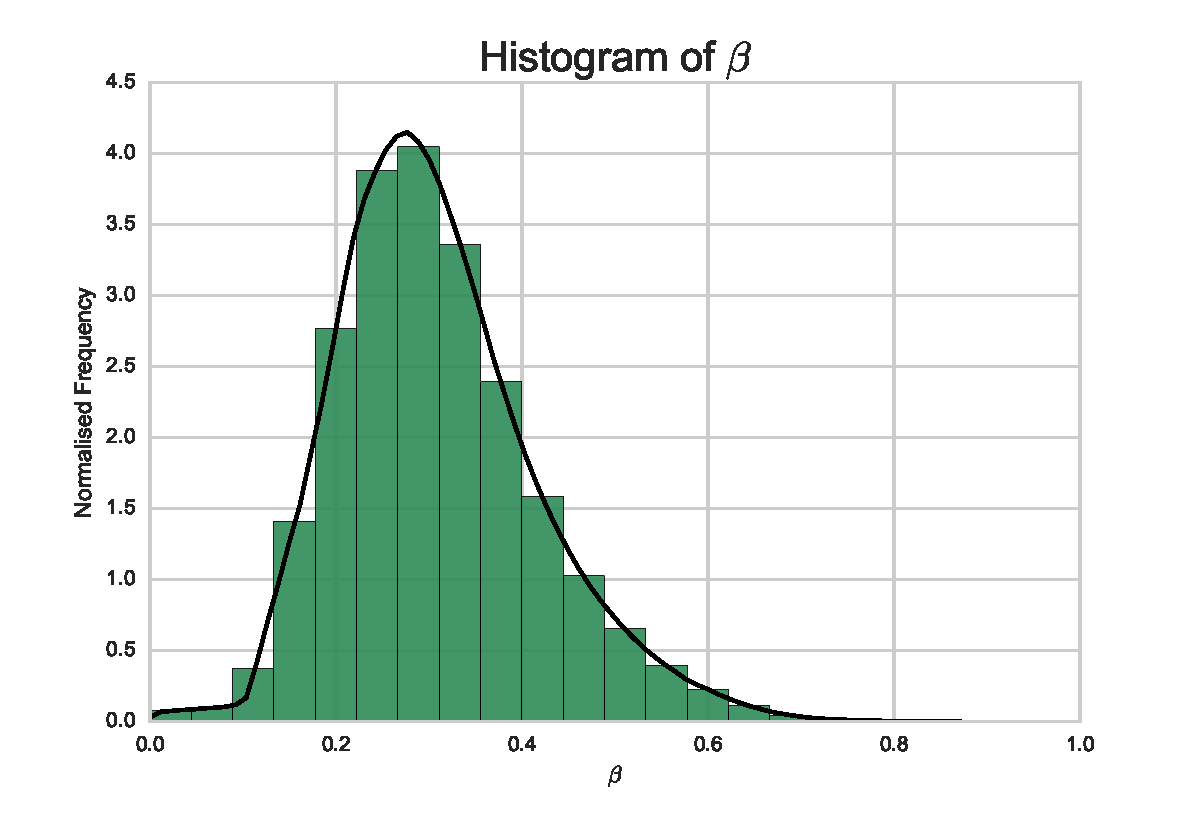
\includegraphics[width=0.5\textwidth]{images/ratio_actual_bound}
  \end{center}
  \caption{Normalised histogram of $\beta$, with estimated pdf.}
  \label{fig:bound_ratio_hist}
\end{figure}

Recalling Section~\ref{sec:markovmodels}, let $p_{(-1)}$, $p_{(-2)}$ and
$p_{(-3)}$ denote the probabilities of $\Omega$ reaching deadlocked state
(-1), (-2) and (-3) respectively, calculated using Equation~\ref{eq:abs_probs}.

Figures~\ref{fig:hexbin_p1} and \ref{fig:hexbin_p3} show hexbin plots with
x-axis $p_{(-1)}$ and $p_{(-3)}$ against the y-axis $\beta$ respectively.
It can be seen that $p_{(-3)}$ has a strong affect on the tightness of the
bound, as the probability of reaching deadlocked state (-3) increases the
bound becomes tighter.
This effect is seems to only begin as the probability increases above
$p_{(-3)} \approx 0.175$.

The probability of reaching deadlock state (-1) does not seem to affect the
tightness of the bound.
The same conclusion can be deduced for $p_{(-2)}$ as the mechanics of the
$\Omega$ system are symmetrical.

\begin{figure}[!htbp]
\begin{subfigure}[b]{0.5\textwidth}
  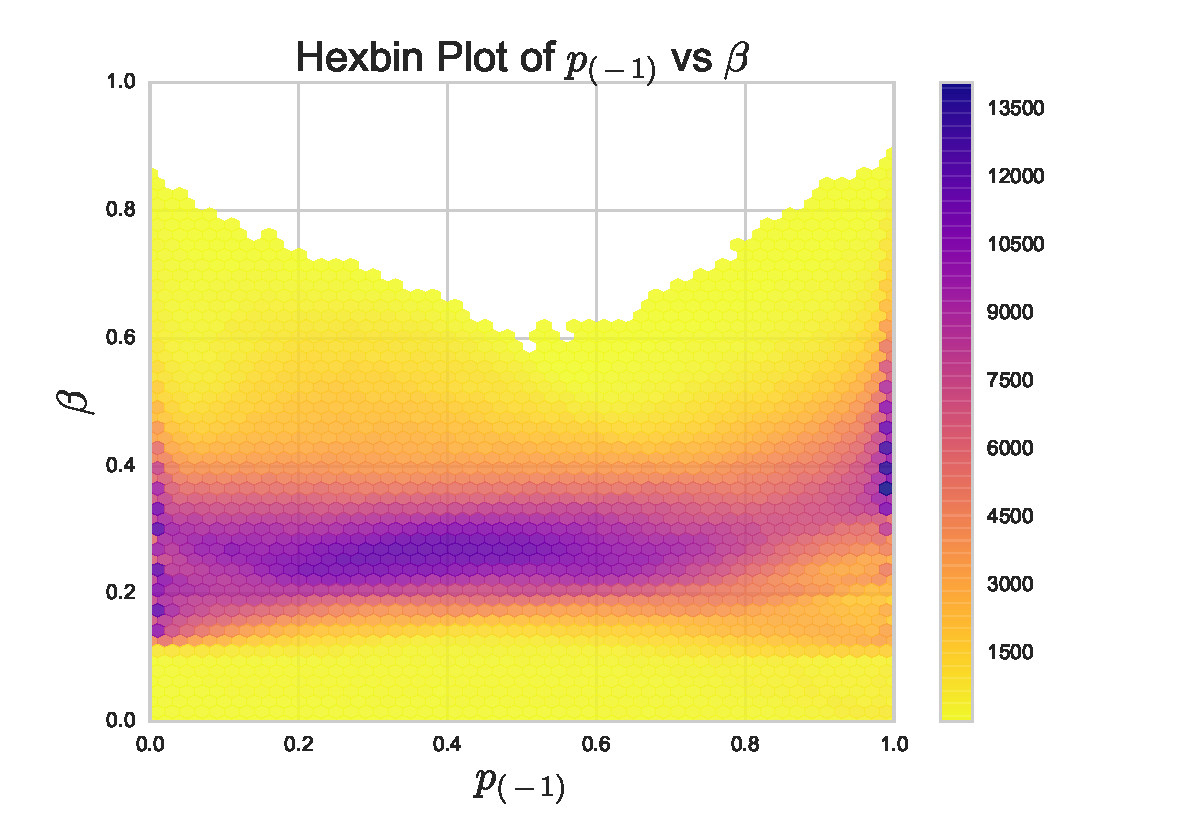
\includegraphics[width=\textwidth]{images/hexbin-1}
  \caption{Hexbin plot of $p_{(-1)}$ against $\beta$.}
  \label{fig:hexbin_p1}
\end{subfigure}
\begin{subfigure}[b]{0.5\textwidth}
  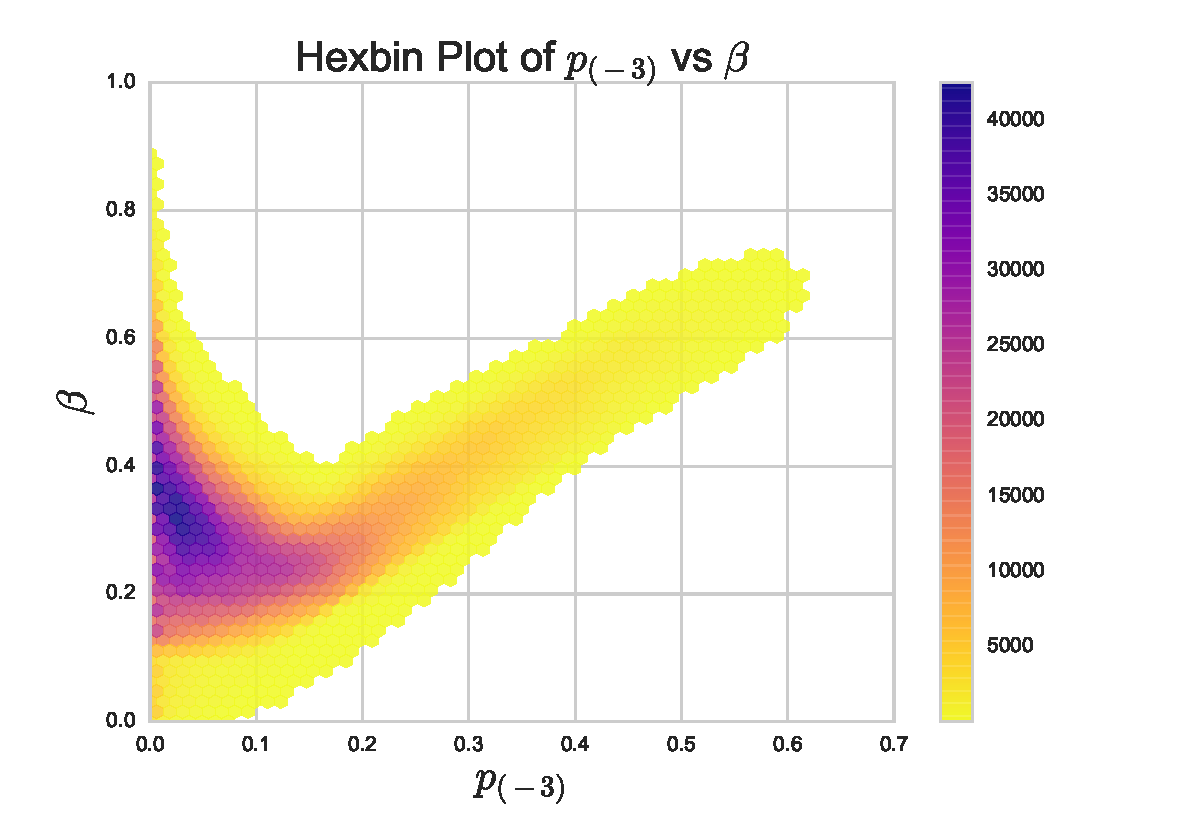
\includegraphics[width=\textwidth]{images/hexbin-3}
  \caption{Hexbin plot of $p_{(-3)}$ against $\beta$.}
  \label{fig:hexbin_p3}
\end{subfigure}
\caption{Hexbin plots of absorption probabilities against $\beta$.}
\label{fig:hexbinplot_ratio_analysis}
\end{figure}

This clearly highlights that the assumptions made about the
$\widetilde{\Omega}_{1_1}$ and $\widetilde{\Omega}_{1_2}$ systems in the proof
of Theorem~\ref{thrm:bound} overestimate the difference between
$\widetilde{\omega}_{1_1}$ and $\omega_{1_1}$, and between
$\widetilde{\omega}_{1_2}$ and $\omega_{1_2}$.
The bound is however tighter for those networks that have a high probability
of reaching deadlocked state (-3).


\section{Conclusions}\label{sec:conclusions}

This paper has explored deadlock in open restricted queueing networks.
It has been shown that analysing a queueing network's corresponding state
digraph is sufficient to detect when deadlock occurs in queueing networks.
In general the presence of a knot in the state digraph will highlight that
deadlock has occurred in the network, however for special cases only the
presence of a weakly connected component with no sink is required.
Incorporating this into a simulation model, time to deadlock can be observed.

Markov models of three deadlocking queueing networks have been built.
Using linear algebraic techniques the expected time to deadlock from each
state was found, and its behaviour as system parameters varied explored.

These analytical results were compared with results obtained from the
simulation model.
Finally a bound on the expected time to deadlock for one of these models was
given, that was found to be tighter for those networks that have high
probability of reaching deadlocked state (-3).

Further research is needed to build a Markov model of the open two node,
multi-server restricted queueing network with routes between nodes and
feedback loops, that is network~\ref{itm:2Nmsf} from Section~\ref{sec:markovmodels}.
In networks~\ref{itm:1Nms} and \ref{itm:2Nmss} customers only have one
potential destination, and so customers may only get blocked from moving to
one destination.
In network~\ref{itm:2Nmsf} with single servers, although customers have two
destinations, a blockage to the same node immediately results in deadlock.
In all these cases, the unblocking mechanism is simple, as there is only ever
one option of which node a customer joins when unblocked.
However in network~\ref{itm:2Nmsf} with multiple servers, there are two
destination nodes to which a customer may join when unblocked.
Therefore, any representations of any states with blocked customers also need
to hold information about these customers' destination nodes.

In addition to this, the order in which customers become blocked is important.
In networks~\ref{itm:1Nms} and \ref{itm:2Nmss} when space become available at
a node there is only one other node from which a blocked customer can become
unblocked, however in network~\ref{itm:2Nmsf} a node that has space available
must accept the customer that has been blocked longest to that node.
Therefore all states with blocked customers are also required to record the
order in which the customers become blocked.
Combining the two requirements above, it is clear that as the number of
servers increases, the size of the state space for this queueing network
quickly grows combinatorially.
Therefore it is not possible to consider this state space in the same way as
for networks~\ref{itm:1Nms} and \ref{itm:2Nmss}.

For the Markov models built in this paper Poisson arrivals and exponential
service rates were assumed, and only blocking of Type I is considered.
A future research direction could be to model other service and arrival
distributions using phase-type distributions, and incorporating these into the
Markov models of deadlocking queueing networks.
Blocking of Type II and III should also be considered, both in the analytical
models and whether the deadlock detection method presented here still holds.
Systems under Type III blocking with random destination (RS-RD) will not reach
deadlock, as there is a non-zero probability of a blocked customer leaving the
system.
This type of blocking may be considered a deadlock prevention mechanism.

The work in Section~\ref{sec:bound}, could be expanded.
Using the ideas presented here it is hoped that a general bound on larger
networks could be found by decomposing the network into smaller known systems.
Thus the ideas could be used to find an upper bound on networks that are yet
to be modelled analytically.

\section{Acknowledgements}

The authors would like to thank and express gratitude to all anonymous
referees whose comments and suggestions have been very helpful.

\bibliographystyle{plain}
\bibliography{refs}

\end{document}
